\documentclass[12pt, a4paper]{article}
\usepackage{pdflscape} %Landscape format

\usepackage{graphicx}
\graphicspath{ {./images/} }

\usepackage[ddmmyyyy]{datetime}
\renewcommand{\dateseparator}{.}
\renewcommand{\figurename}{Şekil}
\renewcommand{\refname}{Kaynaça}
\usepackage{url}
\usepackage{xcolor}
\usepackage{enumitem}
\usepackage{xcolor}
\usepackage{subcaption}
\usepackage{url}
\usepackage{url}
\usepackage{multirow}
\usepackage{colortbl}
\usepackage[table,xcdraw]{xcolor}
\usepackage{array}
\usepackage{xcolor}
\usepackage{subcaption}
\usepackage{amsmath}
\usepackage{hyperref}
\usepackage{cleveref}
\begin{document}
	
	\textbf{KÜTAHYA SAĞLIK BİLİMLERİ ÜNİVERSİTESİ
		MÜHENDİSLİK VE DOĞA BÖLÜMLERİ FAKÜLTESİ}\centering \\[20pt]
	
	\begin{figure}[!h]
		\centering
		
\includegraphics{ksbu.png}
		\\[20pt]
	\end{figure}
	
	\textbf{YAPAY ZEKA DERSİ}\centering\\[10pt]
	
	\textbf{NÖBET ÇİZELGELEME PROBLEMLERİNİN GENETİK ALGORİTMALARLA OPTİMİZASYONU}\centering\\[5pt]
	\textbf{Final Rapor}\\[5pt] 
	\textbf{Mustafa AKER} \\[5pt] 
	\textbf{2118121039} \\[5pt]
	\textbf{\today}\\[20pt]
	\begin{flushleft}
	
	
	\textbf{Özet-Abstract}\\
	Bu çalışmada hemşire çizelgeleme problemi ele alınmıştır. 
	Çizelgeleme çalışmaları bir çok alanda  yaygın olarak kullanılır. İşçilerin ve  makinaların çalışma aralıkalrı ,ders programlarının oluşturulması veya uçakların kalkış iniş saatlerinin belirlenmesinde gibi bir çok alanda cizelgeleme  
	 yapılmaktadır. Ancak sağlık sektöründeki önemi de oldukça 
	büyüktür.. Çizelgelerin elle 
	oluşturulması sorumlu olan kişilerin 6-8 saat kadar zamanını 
	aldığı aşıkardır . Bu koşullar altında bu süreyi minimuma indirecek bir 
	bilgisayar uygulaması şarttır. Çizelgeleme problemleri, çözümü zor olan 
	problemler grubuna girmektedir. Bu nedenle yaklaşık en iyi çözüm değerlerine 
	ulaşabilmek için genetik algoritmalar kullanılmıştır. Çalışma, Buca Seyfi Demirsoy Devlet Hastanesi’nden alınan gerçek 
	verilerle yapılmıştır. Hemşirelerin en uygun 
	çalışma saatlerini bulmak için oluşturulan modelin çözümünde Python programlama  dilinde  
	genetik algoritmalar aracından yararlanılmıştır. Son olarak elde 
	edilen sonuçlar test edilmiş ve tablo şeklinde sunularak çalışma 
	tamamlanmıştır.\\[5pt]
	\textbf{Anahtar  Kelimeler}: Optimizasyon, Genetik Algoritma, Hemşire Çizelgeleme.

	


	\section{Giriş}	
	Sağlık hizmetlerinin temel amacı; kişi, aile ve toplumların sağlıklarının 
	korunması, geliştirilmesi, hasta olanların tedavi edilmesi ve tedavi edilenlerin geri 
	kalan yaşamlarını sağlıklı olarak sürdürülebilmelerini sağlamaktır. İnsanların sağlık 
	hizmetlerinden yeterince, yerinde, zamanında ve gereksiz masraflardan kaçınarak 
	yararlanmaları önemlidir. Ancak bir kurumun 7 gün 24 saat açık olarak hizmet 
	vermesi gerçekten taktiredilmesi gereken bir  çalışmadır. Personelin doğru atanabilmesi büyük bir 
	planlama gerektirir. İşte tüm bu ihtiyaçlar bu çalışmada çizelgelemenin tercih edilmesine 
	sebep olmuştur. . \\[15pt]
	
	
	
	Çizelge (schedule); çizgilerle bölümlere ayrılmış kâğıt anlamına gelir. 
	Çizelge yardımıyla; kadro, kademe, basamak ve derecelerin yer aldığı bir liste elde 
	edilebilir. Çizelgeleme de eldeki işlerin bir grup kaynağa atanmasıdır.\cite{inancc2020solving}\\[15pt]
	
	Çizelgeleme problemleri; en düşük işgücü maliyetleri ile çalışma vardiyalarına 
	atanmaların belirlenmesini, personel hizmet kalitesi ve çalışma yasalarıyla ilgili 
	kısıtlamaların karşılanmasını konu alan problemlerdir.\cite{kuccuk2021hemcsire}\\[15pt]
	
	Çizelgelemedeki asıl amaç, daha az kaynakla ve daha az sürede, 
	istenilen kriterlere uyacak biçimde problemin çözümüne ulaşmaktır.
	Aslında günlük hayatta bir şekilde kişisel not defteri kullanarak yaptığımız planlar da bir çizelge oluşturmaktır. Ancak elbette bir okul, hastane ya da fabrika söz konusu olduğunda değerler 
	büyüyecek ve değişken sayısı artacaktır.Kurumların her türlü unsuru göz önünde bulundurması ve uygun bir çizelge oluşturabilmesi gerekir. Bu sebeple daha kısa sürede bu problemi 
	çözmemizi sağlayacak yollar aranacaktır.\\[15pt]
	
	Sezgisel algoritmalar genellikle en iyiye yakın olan çözüm yoluna hızlı ve kolay bir şekilde ulaştıklarından bu çalışmada sezgisel algoritmalardan olan Genetik Algoritma kullanılmıştır.
	
	
	
	\section{Literatür Araştırması}
	
		\cite{inancc2020solving} 
	İnanç ve Şenaras (2020), evde bakımda hemşire çizelgeleme problemi için 
	Genetik Algoritma kullanmışlardır.\\[10pt]
	
	\cite{kuccuk2021hemcsire} 
	Küçük ve Deveci Kocakoç (2020) hemşirelerin en uygun çalışma saatlerini bulmak icin  MATLAB programının GA aracından yararlanılmıştır\\[10pt]
	
	
	
	
	\cite{yamamura1993nurse}
	90'ların sonlarında sezgisel arama yöntemleri hemşire çizelgeleme için de kullanılmaya 
	başlanmıştır. Yamamura ve diğerlerinin (1993) çalışmaları, GA ile yapılan ilk hemşire 
	çizelgeleme uygulamasıdır.\\[10pt]
	
	\cite{bailey1997using} 
	Bailey ve diğerleri (1997), farklı beceri seviyelerine sahip 
	personelin planlanması sorununa Benzetilmiş Tavlama ve GA uygulamıştır. Sonuçlar, 
	optimal veya optimale yakın çözümler üretilebileceğini göstermektedir.\\[10pt]
	
	
	
	
	\cite{aickelin2004indirect} 
	Aikelin ve diğerlerinin (2004), ele aldıkları yaklaşım, hemşirelerin permütasyonlarına dayanan dolaylı bir kodlama ile programlar oluşturan sezgisel bir kod çözücü kullanmaktır. Sonuçlar, önerilen algoritmanın yüksek	kaliteli çözümler sunabildiğini ve yakın zamanda yayınlanan bir Tabu Arama yaklaşımından daha hızlı ve daha esnek olduğunu ortaya koymaktadır.\\[10pt]
	
	\cite{duenas2009genetic} 
	Duenas ve diğerleri (2009), hemşirelerin tercihlerini içeren çok amaçlı bir 
	çizelgeyi ele almaktadır. Bu tercihler bulanık kümelerle modellenmiştir ve GA ile birleştirilmiş melez bir çözüm yöntemi kullanılmıştır. Sonuçlar, önerilen yaklaşımın iyi kalitede çözümler ürettiğini ve gerçek hayattaki problemlere uygulanabilir olduğunu göstermektedir.\\[10pt] 
	
	
	
	\cite{balekar2013survey} 
	Balekar ve Mhetre (2013), hemşire çizelgeleme	için GA yaklaşımının kullanıldığı çalışmaları toparlayan bir kaynakça sunmuştur.\\[10pt]
	
	\cite{leksakul2014nurse} 
	Leksakul ve Phetsawat çalışmasında elde edilen sonuçlara göre (2014) GA tarafından bulunan hemşire programı,mevcut programla karşılaştırıldığında aylık personel giderlerinde \% 12 ve hemşire sayısında \\ \% 13 tasarruf  görülmüştür.\\[10pt]
	
	
	\cite{kim2018genetic}
	Kim ve diğerleri (2018), popülasyon 
	büyüklüğü ve mutasyon oranı parametrelerini dikkate alarak Memetik Algıritma ve GA 
	kıyaslamışlardır.\\[10pt]
	
	\cite{alfadilla2019optimization} 
	Alfadilla ve diğerleri (2019), acil serviste hemşire çizelgelemesi ile 
	ilgilenmişlerdir. GA hemşirelerin yerine getirilmemiş tercihlerini en aza indirmek için 
	kullanılmaktadır.\\[10pt] 
	

	

	\section{Metodoloji}
	Sezgisel algoritmalar 
	genellikle en iyiye yakın olan çözüm yoluna hızlı ve kolay şekilde ulaştıklarından, çalışmada sezgisel algoritmalardan biri olan Genetik Algoritma (GA) kullanılacaktır. GA, tek çözüm değil birden fazla optimal çözüm elde etmesi, çok sayıda parametre ile çalışma imkanı olması, amaç fonksiyonunu geniş bir açıda araştırması nedeniyle yararlı bir yöntemdir. 
	\\[5pt]
	
	\subsection{Genetik Algoritma }
		Evrimsel hesaplamanın bir alt dalı olan genetik algoritmalar, yapay zekânın 
	hızla gelişen alanlarından biridir. Bu metasezigel yaklaşımların 
	esin kaynağı Darwin’in evrim teorisidir. Evrimsel hesaplama kavramı, 1960’lı 
	yıllarda I.Rechenberg’in “Evrim Stratejileri” adlı çalışmasında ortaya atılmıştır. 
	Takip eden 1970’li yıllarda da Michigan Üniversitesi’nden John Holand tarafından 
	genetik algoritmalar bulunmuş ve öğrencileri ile meslektaşları yardımıyla 
	geliştirilmiştir. Bunu 1975 yılında Holland’ın “Doğal ve Yapay Sistemlerde Uyum”
	adlı kitabını yayınlaması izlemiştir.\\[5pt]
	Genetik algoritmalar konusundaki esas gelişim ise, John Holland’ın doktora 
	öğrencisi David E. Goldberg tarafından 1985 yılında hazırlanan “Gaz ve Boru 
	Hatlarının Genetik Algoritma Kullanılarak Denetlenmesi” konulu doktora tezi ile 
	sağlanmıştır. Ulusal Bilim Fonu tarafından verilen Genç Araştırmacı Ödülü’nü 
	kazanan Goldberg, dört yıl sonra 1989 yılında yayımladığı “Makine Öğrenmesi, 
	Arama ve Optimizasyon İçin Genetik Algoritma” adlı kitabı ile genetik algoritmaya 
	yeni bir boyut kazandırmıştır. Bu çalışma günümüzde dahi genetik algoritma 
	konusunda en kapsamlı referans olma özelliğindedir.\\[5pt]
	Genetik algoritma yöntemi, evrim teorisi esaslarına göre çalışarak, verilen bir 
	sorun için en iyi çözüm veya çözümleri bulmaya yarar. Bu arayışı, karar değişkeni 
	uzayındaki birçok başlangıç noktasından başlayarak, paralel işlemler dizisi ile en iyi 
	yöne doğru gelişerek yapar. Karar uzayındaki bu noktalarda uygunluk derecelerinden 
	başka bilgilere gerek yoktur. Toplumdaki noktaların paralel çalışarak en iyiye doğru 
	gelişmesi rastgelelik ilkeleri ile sağlanmaktadır. Genetik algoritmanın esası doğal seçme ve genetik kurallarına dayanmaktadır. Bu kurallar ortama en fazla uyum sağlayan canlıların hayata devam etmesi ve uyum sağlayamayanların da elenmesi olarak algılanmalıdır.\\[5pt]
	Genetik algoritmalar doğadaki en iyinin yaşamasını 
	gerektirmekte ve bunu belirleyen uygunluk işlevi, yeni çözümler üretmek için 
	çaprazlama, kopyalama ve değiştirme gibi operatörleri kullanmaktadır. Genetik 
	algoritmanın önemli özelliklerinden birisi de bir grup üzerinde çözümü araması ve bu 
	sayede çok sayıda çözümün içinden en iyiyi seçmesidir.\\[10pt]
	
	Probleme ait en iyi çözümün bulunabilmesi için; 
	\begin{enumerate}
		\item {Bireylerin gösterimi doğru bir şekilde yapılmalı,}
		\item {Uygunluk fonksiyonu etkin bir şekilde oluşturulmalı,}
		\item { Doğru genetik işlemciler seçilmelidir,}
	\end{enumerate}
	
	
		\subsection{Genetik Algoritmaların Diğer Yöntemlerden Farkı}
	Goldberg’e göre genetik algoritmayı diğer arama yöntemlerinden ayıran en 
	belirgin özellikleri çözüm arama şeklinin farklı oluşudur.
	\begin{enumerate}
		\item {Genetik algoritma, parametre setlerinin kodları ile ilgilenir, parametrelerin 
			kendileri ile doğrudan ilgilenmez,}
		\item {Genetik algoritmanın arama alanı, yığının veya populasyonun tamamıdır; 
			tek nokta veya noktalarda arama yapmaz, }
		\item {Genetik algoritmalarda, amaç fonksiyonu kullanılır, sapma değerleri veya 
			diğer hata faktörleri kullanılmaz, }
		\item {Genetik algoritmaların uygulanmasında kullanılan operatörler, stokastik 
			yöntemlere dayanır, deterministik yöntemler kullanılmaz}
	\end{enumerate}
	Başka bir ifadeyle genetik algoritmalar doğal olayların gelişmesindeki 
	genetik mekanik ilkelere göre çalışırlar.
	\begin{itemize}
		\item {Genetik algoritmalar, çözümlemesinde karar değişkenlerini genetik sayı 
			sistemine göre kodlayarak kullanır. Sayı sisteminde karar değişkenlerinin genleri 
			topluca karar uzayında bir noktayı temsil eder.}
		\item {Genetik algoritmalarda bir nokta yerine aynı anda noktalar topluluğundan 
			hareket edilir. Topluluğun genetik algoritmalar evrimi ile gelişmesi sonucunda en iyi 
			çözüme ulaşılır. Evrim sırasında sistem yerel en iyiye takılmaz}
		\item {Genetik algoritmalar evrimi sırasında, karar değişkenlerinin belirttiği 
			noktalardaki hedef fonksiyonu değerleri kullanılır. Türev ve integral işlemlerine 
			gerek olmadığından başlangıç ve sınır şartları ile bazı klasik kabullerin yapılmasına 
			gerek yoktur}		
		\item{Genetik algoritmalar evrim işlemleri belirlilik değil kurallarına dayanır. 
			Seçim işlemleri ihtimal ilkeleri ışığı altında yapılır. En iyi için sayılan klasik 
			yöntemlerin dışında daha basit, fazla matematik gerektirmeyen ve objektif olan GA
			(genetik algoritma) yaklaşımları kullanılabilir. Genetik algoritmalardaki rastgele 
			yaklaşımlar sonuç çözümün yerel en iyi çözümlere takılıp kalmamasını sağlar}	
	\end{itemize}
	
	\subsection{Temel Kavramlar}\cite{kuccuk2021hemcsire}
	Genetik algoritmanın çalışmasında ve başarılı çözüm değerlerine 
	ulaşılmasında temel kavramların iyi anlaşılmasının ve belirlenmisinin önemi 
	büyüktür.
	\subsubsection{ Gen}
	Kalıtsal molekülde bulunan ve organizmanın karakterlerinin tayininde rol 
	oynayan kalıtsal birimlere denir. Yapay sistemlerde gen, kendi başına anlamlı birer 
	genetik bilgi taşıyan en küçük yapı birimi olarak alınır.\\[5pt]
	Genetik algoritmanın kullanıldığı programlama yapısında bu gen yapıları 
	programcının tanımlamasına bağlıdır. Bir genin içerdiği bilgi sadece ikili tabandaki 
	sayıları içerebileceği gibi onluk taban ve onaltılık tabandaki sayı değerlerini de 
	içerebilir. Dolayısıyla yazılan programa göre gen içeriği çok önem kazanmaktadır
	\subsubsection{  Kromozom}
	Bir ya da birden fazla gen yapısının bir araya gelerek oluşturduğu problemin 
	çözümüne ait tüm bilgiyi içeren diziye kromozom denir. Kromozomlar, alternatif 
	aday çözümleri gösterirler \\[5pt]
	Kromozornlann bir araya gelmesiyle populasyon (yığın) oluşturulur. 
	Yığındaki her bir bireye kromozom, kromozomdaki her bir bilgiye gen denir. 
	Kromozomlar, üzerinde durulan problemin olası çözüm bilgilerini içermekledir 
	Kromozom, GA yaklaşımında üzerinde durulan en önemli birim 
	olduğu için bilgisayar ortamında iyi ifade edilmesi gerekir.
	
	\subsubsection{  Populasyon}
	
	Populasyon, çözüm bilgilerini içeren kromozomların bir araya gelmesiyle 
	oluşan olası çözüm yığınına denir. Yığındaki kromozoın sayısı sabit olup problemin 
	özelliğine göre programlayıcı tarafından belirlenir .\\[5pt]
	Çözüm uzayı açısından populasyon büyüklüğünün küçük değerde olması 
	çözüm uzayının küçük olmasını bu da aranan en iyi çözüm değerlerine 
	ulaşılamamasına neden olmaktadır. Çözüm uzayının çok büyük değerde olması ise 
	hem genetik algoritmanın etkinliğini azaltmakta hem de çözümün farklı noktalarda 
	aranmasına neden olmaktadır .\\[5pt]
	
	
	
	\begin{figure}[h]
		\item {Gen, Kromozom ve Populasyon Yapısı}
		\centering
		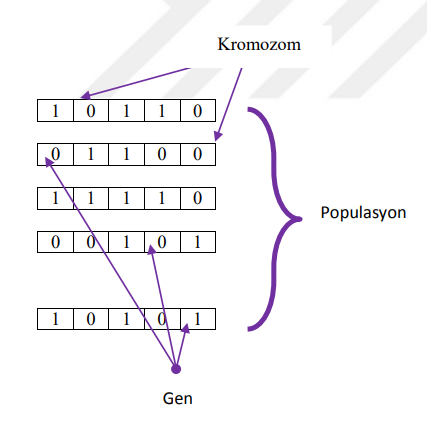
\includegraphics{gen.png}
		\\[20pt]
	\end{figure}
	
	\subsection{Kodlama}
	İlk adım; problem için arama uzayını en iyi temsil eden kodlama yapısının 
	seçilmiş olmasıdır. Kodlama biçimi, genetik algorimanın performansını oldukça önemli oranda etkiler; fakat programa bağlı olduğundan bütün problemler için geçerli en uygun kodlama biçimini söylemek imkânsızdır\\[5pt]
	\subsubsection{İkili (Binary) Kodlama}
	En yaygın olarak kullanılan kodlama türüdür. Burada kromozomlar 0 ve 1 
	şeklinde gen değerlerinde kodlanırlar. Bu dizideki her bit, çözümün belli
	karakteristiğini temsil eder veya tüm dizi bir sayıyı temsil eder. 
	
		\begin{figure}[h]
		\item { İkili Düzende Kodlama Yapısı}
		\centering
		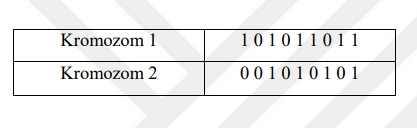
\includegraphics{iki.png}
		
	\end{figure}
	
	\subsubsection{ Sıralı (Permütasyon) Kodlama}
	Sıralı (permütasyon) kodlama tekniği genellikle gezgin satıcı, çizelgeleme ve 
	sıralama, şebeke tasarımları gibi sıra takibi olan problemlere uygulanır.
	
	\begin{figure}[h]
		
		\centering
		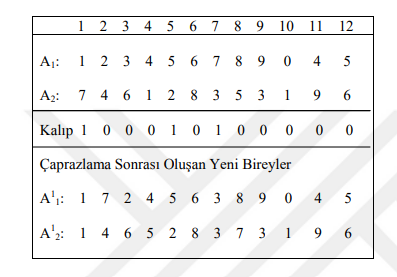
\includegraphics{sıralı.png}
		
	\end{figure}
	
	\subsubsection{Değer (Alpha-Numeric Encoding) Kodlaması}
	Değer kodlama yönteminde ilgili parametre değerleri doğrudan alınır. Özel
	problemlerde alfa-sayısal ya da gerçel sayılar olarak kullanımı gerçekleştirilir
	
	\begin{figure}[h]
		\item { Değer kodlama yapısı}
		\centering
		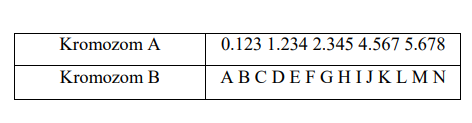
\includegraphics{deger.png}
		
	\end{figure}
	

	\subsection{ Seçim}
	Goldberg’e göre, yeni nesiller için ebeveyn kromozomların belirlenmesi 
	sürecinde önceki populasyondan gelen bazı kromozomların yeni populasyona 
	aktırılması gerekmektedir. Burada önemli olan bu kromozomların nasıl seçileceğidir. 
	Darvin evrim teorisine göre; hayatta kalan en iyi kromozom ebeveyn olarak yeni 
	oğul kromozomları oluşturur. En iyi kromozom seçilmesinde birçok yöntem 
	bulunmaktadır. Her bir kromozomun uygunluk değeri hesaplandıktan sonra 
	uygunluğu yüksek olan kromozomların seçilmesi için geliştirilmiş değişik seçim
	yöntemleri bulunmaktadır
	
	\subsubsection{Rulet Tekeri Seçim Yöntemi}
	Genetik algoritmalarda kullanılan en basit ve en yaygın seçim mekanizması 
	rulet tekerleği (çemberi) seçimidir. \\[2pt]
	Rulet Tekeri seçim operatöründe, bütün kromozomlar uygunluk değerlerine 
	göre bir rulet etrafında dizilirler. Rulet üzerinde uygunluk değerlerine göre sıralanan 
	kromozomlar rasgele olarak seçilirler. Bu şekilde her birey seçilmek için kendi 
	uygunluk değerine göre bu rulet tekerinden bir pay almaktadır. Daha büyük alana 
	sahip bireyin seçilme şansı daha fazla olacaktır. Bu metot yardımıyla kromozomlar 
	istatistiksel yöntemler kullanılarak uygunluk fonksiyonu değerlerinin toplam 
	uygunluk fonksiyonuna oranları ölçüsünde seçilirler. Ancak bu seçim yöntemi, uyum 
	değeri büyük olan bireylerin seçilme olasılığı yüksek olduğu için hep aynı 
	kromozomların seçilmesine neden olmaktadır. Bu da populasyon içindeki çeşitliliği 
	etkileyerek sorun yaratır.
	
	\begin{figure}[h]
		\item { Rulet Tekerleği Seçme Operatörü}
		\centering
		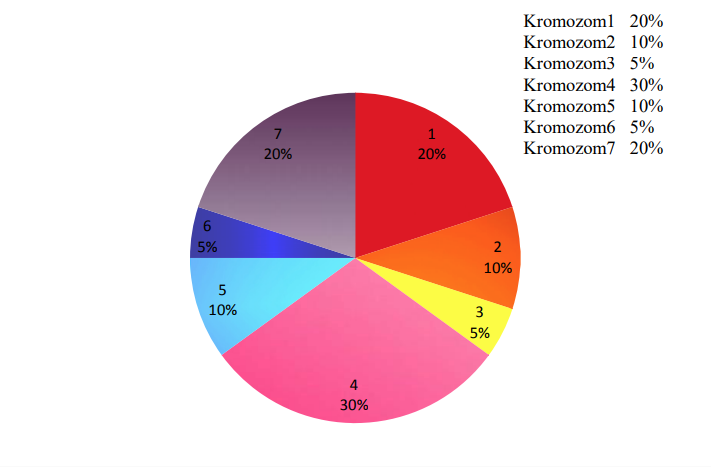
\includegraphics[width=0.9\textwidth]{rulet.png}
	
	\end{figure}
	
	\newpage
		\subsubsection{Sıralı (Rank) Seçim Yöntemi}
	Rulet seçimi eğer uyumluluk çok fazla değişiyorsa sorun çıkartabilir. Örneğin 
	en iyi kromozomun uyumluluğu \%90 ise diğer kromozomların seçilme şansı 
	azalacaktır. Bunu önlemek için sıralı seçim kullanılabilir. Sıralı seçimde en kötü 
	uyumlulukta olan kromozoma 1 değeri sonrakine 2 değeri verilir ve böylelikle 
	seçilmede bunlara öncelik tanınmış olur. Bu şekilde onların da seçilme şansı artar. 
	Fakat bu da çözümün daha geç yakınsamasına neden olabilir\cite{holland1992adaptation}
	
	\begin{figure}[h]
		\item {Sıralı Seçim}
		\centering
		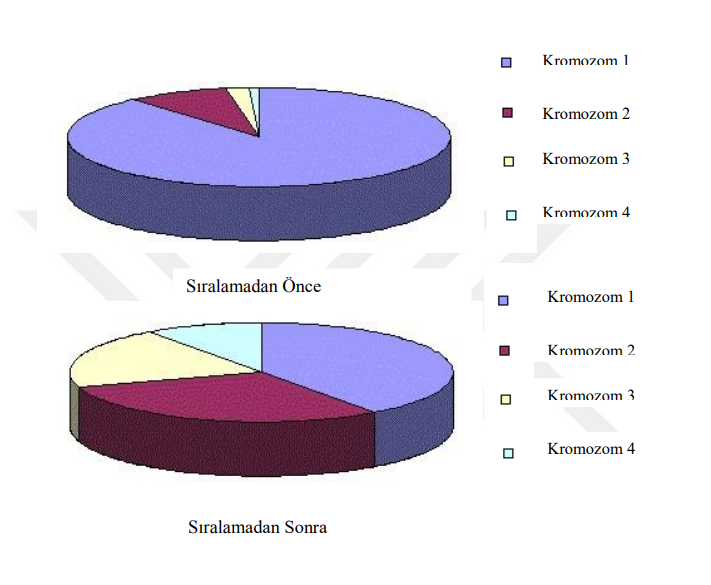
\includegraphics[width=0.9\textwidth]{sıralı.secim.png}
		\\[20pt]
	\end{figure}
	
	\newpage
	\subsubsection{ Turnuva Seçim Yöntemi}
	
	Bu seçim yönteminde, bireyler rasgele olarak gruplanır ve gruptaki bireyler 
	aralarında seçim işlemi yapılmak üzere rekabete sokulur. Grup içinde en yüksek 
	uygunluk değerine sahip olan birey, yeni nesli oluşturmak için ebeveyn bireylerden 
	biri olarak seçilir. Bu işlem, toplam birey sayısına ulaşıncaya kadar devam eder. Bazı 
	uygulamalarda grup büyüklüğü iki olarak seçilirken, bazılarında çok daha büyük 
	gruplar oluşturulur \cite{elen2011ccizelgeleme}
	
	\begin{figure}[h]
		\item {Turnuva Seçim Yöntemi}
		\centering
		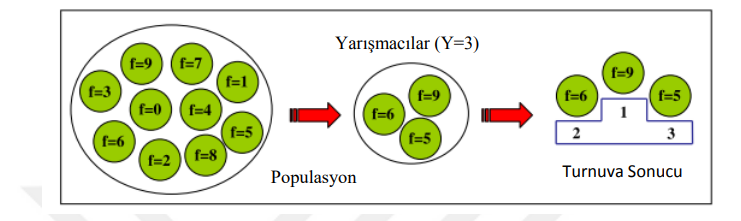
\includegraphics{truva.png}
		
	\end{figure}
	\item {Populasyondaki bireylerin uygunluk değerleri f ile bireyler arasından rasgele seçilen grup büyüklüğü 
		Y ile gösterilmiştir}
	
	
	
	\subsubsection{ Sabit Durum (Kararlı Hal) Seçim Yöntemi}
	Sabit durum metodunda, her nesilde yalnızca birkaç birey yer değiştirir. 
	Çoğunlukla çok düşük uygunluk değerine sahip bireyler, çaprazlama ve mutasyon 
	yöntemleriyle yeniden üretilerek yeni nesilde yer alırlar. Sabit durumlu GA’lar daha 
	çok kural tabanlı sistemlerde kullanılır
	
	\subsubsection{Seçkinlik (Elitizm) İşlemi}
	Mansfield’e göre üreme, çaprazlama ve mutasyon işlemleri sonrasında 
	kuşakta bulunan en iyi uygunluk değerine sahip birey, sonraki kuşağa 
	aktarılamayabilir. Bunu önlemek için bu işlemlerden sonra oluşan yeni kuşağa bir 
	önceki kuşağın en iyi (elit) bireyi, yeni kuşaktaki herhangi bir birey ile değiştirilir. 
	
	
	\newpage
	\subsection{ Genetik Operatörler}
	Genetik algoritmalarda belirli noktalardan sonra nesil çeşitliliği 
	olmamaktadır. Bunun için dizilere çaprazlama (crossing over) ve değişim (mutation) 
	operatörleri belirli yüzdelik oranlarıyla uygulanarak nesil çeşitliliği sağlanır. Böylece 
	çözümün belirli noktalara gelip tıkanması önlenmiş olur\\[5pt]
	
	\subsubsection{ Çaprazlama}\cite{birougul2005genetik} \\[5pt]	
	
	Çaprazlama ebeveynlerden bazı genleri alarak yeni bireyler oluşturma 
	işlemidir. Burada amaç, eldeki nesilden farklı nesiller elde etmektir. Çaprazlama
	yapılacak konum rastgele seçilir. Oluşan yeni birey ebeveynlerin bazı özelliklerini 
	almış ve bir bakıma ikisinin kopyası olmuştur. Daha iyi performans almak amacıyla 
	değişik çaprazlamalar kullanılabilir\\[5pt]
	
	
	\begin{figure}[h]
		
		\centering
		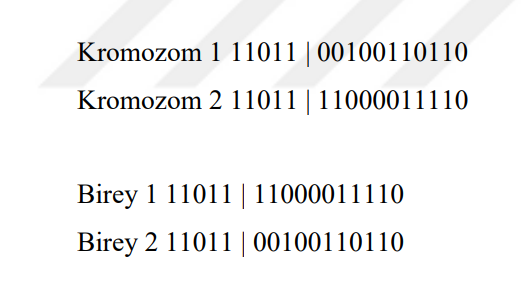
\includegraphics[width=0.9\textwidth]{cap.png}
		\\[20pt]
	\end{figure}
	
	Çaprazlama operatörü, iki dizinin bir araya gelerek karşılıklı gen yapılarının 
	değişimi ile yeni dizilerin oluşumunu sağlayan operatördür. Çaprazlanarak gen 
	değişiminin yapılmasından önce dizilerin çaprazlamaya tutulma olasılığı 
	belirlenmelidir. Literatürde bu oranın \%50-\%95 oranında uygulandığı görülmektedir.\\[5pt]
	Çaprazlamada bir diğer önemli unsur ise ne tür bir 
	çaprazlamanın yapılacağıdır.
	
	\subsubsection{İkili kodlama Düzeninde Çaprazlama Yöntemleri}
	İkili kodlama düzeni için çaprazlama yöntemleri tek nokta, iki nokta ve üç
	nokta çaprazlama yöntemleri olarak sınıflandırılmıştı.
	\begin{itemize}
		\item  \textbf {Tek Nokta Çaprazlama Operatörü:} \\
		Bu işlemde kromozomlar rastgele bir yerinden kesilir ve sonra ilgili genler ile yer değiştirilir.
		\begin{figure}[h]
			{ Tek Noktalı Çaprazlama} 
			\centering
			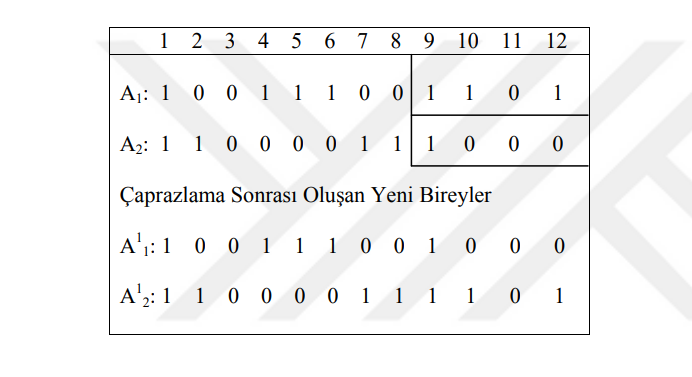
\includegraphics{teknokta.png}
			\\[20pt]
		\end{figure}\cite{birougul2005genetik}
		\clearpage
		\item  \textbf {İki Nokta Çaprazlama Operatörü:} \\
		Bazı durumlarda tek noktalı çaprazlama yöntemi yetersiz kalabilir ya da büyük parçalı blokların bozulması performansı düşürebilir. Bu sebeple iki noktalı çaprazlama yöntemi tercih edilebilir.İki noktalı çaprazlama operatöründe, rasgele iki nokta seçilir ve bu iki nokta arasında 
		kalan bloklar kromozomlar arasında yer değiştirilir. Bu yöntem populasyondaki kromozomların performansını arttırabilir.\cite{elen2011ccizelgeleme}
		\begin{figure}[h]
			{ İki Noktalı Çaprazlama}
			\centering
			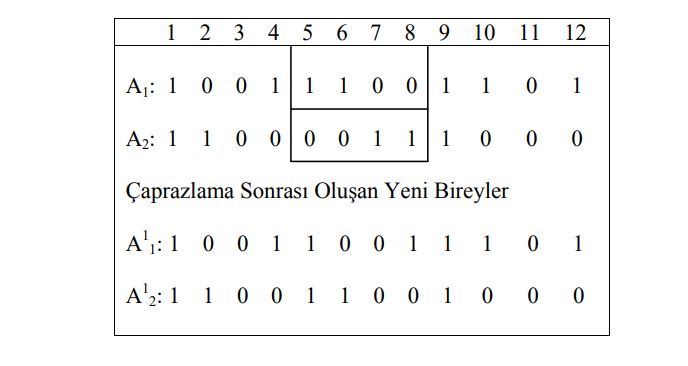
\includegraphics{ikinokta.png}
			\\[20pt]
		\end{figure}
		
	\end{itemize}
	
	\subsubsection{Sıralı Kodlama Düzeninde Çaprazlama Yöntemleri}
	Çizelgeleme problemlerinde sıkça kullanılan sıralı (permütasyon) kodlama 
	düzeninde yer alan çeşitli çaprazlama yöntemleri mevcuttur\clearpage
	\begin{itemize}
		\item \textbf{ Pozisyona dayalı çaprazlama operatörü (PBX):}
		bu yöntemde 
		çaprazlama kalıp olarak sabit kalacak olan gen hücrelerini belirler. Kalıpla 
		işaretlenen noktalar dizide sabit kalırken diğer noktalarda iki birey yer değiştirilerek 
		yeni bireylerin üremesi sağlanır.\cite{aydemir2009atolye}
		\begin{figure}[h]
			{ Pozisyona Dayalı Çaprazlama} 
			\centering
			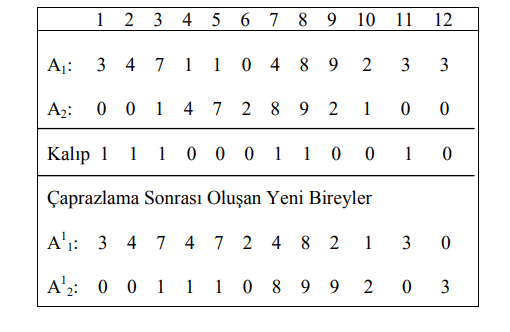
\includegraphics{pozisyon.png}
			
		\end{figure}
		\item \textbf{Sıraya dayalı çaprazlama operatörü (OBX):}
		kalıp üzerindeki 1 değerleri çaprazlamada kullanılacak değerleri gösterir. Bu tür çaprazlama, 
		kromozomu oluşturan karakterlerin sayı ve sıralarının önem taşıdığı durumlarda 
		kullanılır.
		\begin{figure}[h]
			\ {Sıraya Dayalı Çaprazlama} \\[5pt]
			\centering
			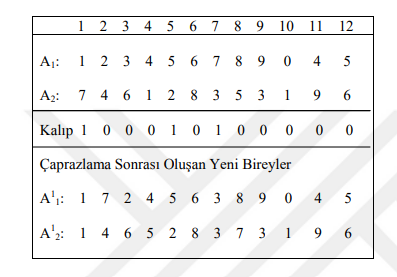
\includegraphics{sıralı.png}
			\\[20pt]
		\end{figure}
		
		\item \textbf{Kısmi eşleşmeli çaprazlama operatörü (PMX):}iki bireyden rastgele bir 
		aralık belirlenir. Bu aralıktaki değerler yer değiştirilir
		\begin{figure}[h]
			\ { Kısmi Planlı Çaprazlama} \\[5pt]
			\centering
			\includegraphics{kısmi.png}
			\\[10pt]
		\end{figure}\\
		Yer değiştirme sonunda dizide aynı olan değerler değiştirilen değerlerle tamamlanır. 
		\begin{figure}[h]
			
			\centering
			\includegraphics{kısmi2.png}
			\\[10pt]
		\end{figure}
	\end{itemize}
	\newpage
	\subsection{ Mutasyon}\cite{kuccuk2021hemcsire}\\
	Kromozomların genleri veya genleri oluşturan küçük birimleri üzerinde 
	değişiklik yapılmasını sağlayan işlemcidir. Değişime uğratılacak kromozomun 
	seçiminde, kromozomun değişime uğrama ihtimalini gösteren ve başlangıçta sabit 
	olarak tanımlanan bir değişim oranı söz konusudur. Genetik algoritmalarda değişime
	tabi tutulacak kromozomların belirlenmesinde bazılarının istisna tutulması veya 
	özellikle değişime uğratılması gibi özel stratejiler tanımlanabilir.\\[5pt]
	
	Amaç belli bir nesil sayısından sonra populasyon içerisindeki bireylerin 
	gitgide birbirlerine benzemesine engel olmaktır. Çünkü bu durum çözüm uzayının 
	daralmasına neden olmaktadır. Bireylere ne kadar çaprazlama operatörü uygulansa 
	da belli bir nesil sayısından sonra birey çeşitliliği sağlanmamaktadır. Bu durumda 
	bireyi oluşturan genlerden rasgele bir tanesi seçilir. Rasgele seçilen genin değeri 
	değiştirilir. Böylelikle populasyon içindeki bireylerin çeşitliliğinin devamı sağlanmış
	olunur . Yapay sistemlerde mutasyon işlemi esnasında kromozomdaki 
	gen sayısı değişmez sabit kalır. Doğal populasyondaki mutasyon oranı oldukça 
	düşüktür. Mutasyon frekansının büyüklüğü GA’nın performansını etkilemektedir. 
	Mutasyon işlemi bir tek kromozom üzerinde yapılır\\[5pt]
	
	Mutasyon oranı, tıpkı çaprazlama oranında olduğu gibi mutasyonun 
	olasılığını ifade eden bir orandır. Yine rasgele yöntemlerle kromozomun mutasyona
	uğrayıp uğramayacağı belirlenir ve buna göre mutasyon gerçekleştirilir. Mutasyon 
	oranı genellikle çok düşük (0,01) olduğundan mutasyon işlemi fertlerde az görülür 
	. \\[5pt]
	Mutasyonun sağladığı avantaj, problemin çözüm alanını araştırmada yön 
	değişikliklerini sağlayarak araştırmanın kısır döngüye girmesini önlemektir. Mutasyon yöntemleri genel olarak beş farklı şekilde sınıflandırılmıştır \\[5pt]
	
	
	\subsubsection{  Ters Mutasyon}
	
	Bir bireyde rassal olarak iki pozisyon seçilir, bu iki pozisyondaki alt diziler 
	ters çevrilir
	
	\begin{figure}[h]
		{ Ters Mutasyon}
		\centering
		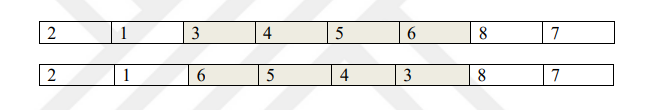
\includegraphics{ters.png}
		\\[10pt]
	\end{figure}
	\newpage
	\subsubsection{Komşu İki Geni Değiştirme}
	Rassal olarak iki komşu iş yer değiştirebilir.
	
	\begin{figure}[h]
		{ Komşu İki Geni Değiştirme}
		\centering
		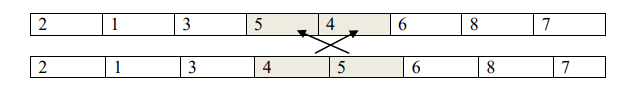
\includegraphics{komsu.png}
		\\[10pt]
	\end{figure}
	
	\subsubsection{Keyfi İki Gen Değiştirme}	
	Rassal olarak seçilen iki iş değiştirilebilir. Özel bir durum olarak, 
	değiştirilebilen iki komşu işi bu mutasyon içerir
	\begin{figure}[h]
		{ Keyfi İki Gen Değiştirme}
		\centering
		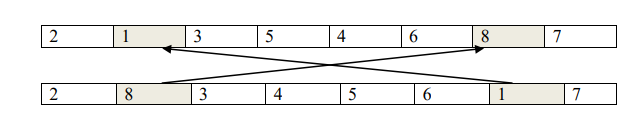
\includegraphics{keyfi.png}
		\\[10pt]
	\end{figure}
	
	\subsubsection{Keyfi Üç Gen Değiştirme}	
	Rassal seçilen üç iş keyfi olarak değiştirilir
	\begin{figure}[h]
		{  Keyfi Üç Gen Değiştirme}
		\centering
		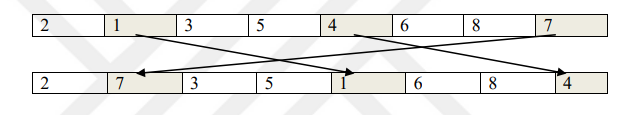
\includegraphics{keyfi3.png}
		\\[10pt]
	\end{figure}	\newpage	
	\subsubsection{Araya Yerleştirme}	
	Rassal olarak seçilen bir kaydırma noktasında kromozomdaki bir iş kaydırılır 
	ve diğer bir pozisyona yerleştirilir. Komşu iki iş değiştirme yönteminin özel bir 
	durumudur. Keyfi üç iş değiştirmeyle bir kesişime sahiptir
	\begin{figure}[h]
		{   Araya Yerleştirme}
		\centering
		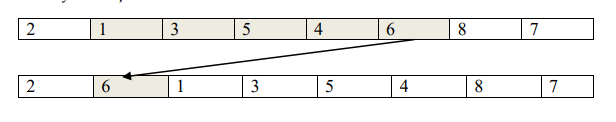
\includegraphics{ara.png}
		\\[10pt]
	\end{figure}
	
	\subsection{ Durdurma Kriteri}
	Üreme, çaprazlama ve mutasyon işlemlerinden sonra yeni bir nesil
	oluşmaktadır. Tüm bu işlemler sonsuz döngü içerisinde yapılır. Eğer bir durdurma 
	kriteri belirlenmez ise bu süreç sonsuza kadar devam eder.
	\begin{enumerate}[label=\Alph*.]
		\item \textbf{Hesaplama zamanı kriteri:}\\
		Bu yöntemde önceden bir hesaplama zamanı 
		veya döngü sayısı belirlenmekte, bu zaman veya döngü sayısına ulaşıldığında 
		durdurulmaktadır. Bu yöntemde belirlenen döngü sayısı gerektiğinden fazla ya da 
		eksik olabilir.
		\item \textbf{ Optimizasyon hedefi kriteri:}\\
		Önceden ulaşılması istenen amaç fonksiyonu 
		değeri bilinmektedir. Uyum değeri bu değere ulaştığında algoritma 
		durdurulmaktadır.
		\item \textbf{Minimum iyileşme kriteri:}\\
		Genetik algoritma problemlerinde bulunan en iyi 
		çözümler önce hızlı daha sonra yavaş yavaş artış göstermektedir. Bulunan 
		değerlerdeki iyileşme hızının giderek azalması ve sıfıra yaklaşması, artık daha fazla 
		iyileşme beklenmemesi gerektiğini gösterebilir. Çözüme harcanacak zaman ile 
		çözümden beklenecek kalite arasında bir denge kurularak durdurma gerçekleştirilir\cite{birougul2005genetik} \\[5pt]
	\end{enumerate}
	
	
	\subsection{Genetik Algoritmaların Çözümünde Takip Edilecek İşlem 
		Adımları}
	\begin{enumerate}
		\item Adım 1: Kullanıcının önceden tanımladığı kurallara göre genellikle rassal bir 
		çözüm grubu seçilir veya kullanıcının kendisi ilk çözüm grubunu belirleyebilir. İlk 
		çözüm grubuna başlangıç populasyonu denir.
		\item Adım 2: Her bir kromozom için bir uygunluk değeri hesaplanır; bulunan 
		uygunluk değerleri dizilerin çözüm kalitesini gösterir. Populasyonda yer alan en iyi 
		uygunluk değerine sahip olan birey (kromozom), bir sonraki yeni nesile (populasyon) 
		doğrudan değiştirilmeden aktarılır. 
		\item	Adım 3: İki grup dizi (kromozom), belirli bir seçim yöntemine (uygunluk 
		değerlerine) göre rassal olarak seçilir. 
		\item	Adım 4: Seçilen iki kromozom için rassal olarak genetik operatörler 
		kullanılarak çaprazlama işlemi gerçekleştirilir. Sonuçta yeni populasyonda yer alacak 
		iki yeni birey (kromozom) oluşur. Çaprazlama, yeni populasyonda yer alacak birey 
		sayısına ulaşılana dek sürer. 
		\item	Adım 5: Yeni populasyondaki bireyler, rassal olarak mutasyon işleminden 
		geçerler.
		\item	Adım 6: Önceden belirlenen nesil sayısı boyunca yukarıdaki işlemler 
		sürdürülür. Eğer en büyük nesil sayısına ulaşılmamışsa Adım 2’ye dönülür. En 
		büyük nesil sayısına ulaşınca işlem bitirilir. Uygunluk değeri en yüksek olan 
		kromozom (çözüm) seçilir.
	\end{enumerate}
	\newpage
	\begin{figure}[h]
		\item { Genetik Algoritmanın Akış Diyagramı} \cite{birougul2005genetik} \\[5pt]
		\centering
		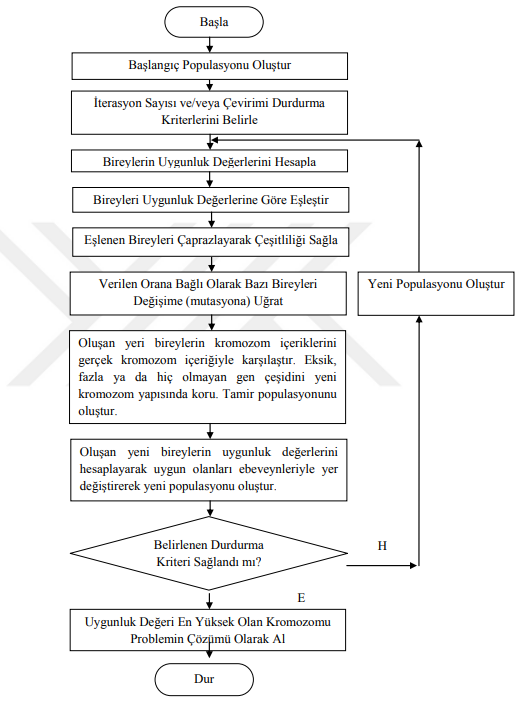
\includegraphics{sema.png}
		\\[20pt]
	\end{figure}
	
	\clearpage
	\subsection{Yapılan Çalışmalar}
	Bu bölümden yukarıda anlatılan  Genetik Algoritma kavramlarını anlaşılması icin  basit  uygulamalar yapılmıştır.
	\subsubsection{Örnek-1}\cite{mıracöztürk}
	
	Uygulamada ki amac belirli bir bit dizisi (hedef gen) oluşturmaktır.\\
	Başlangıçta rastgele bir popülasyon oluşturulur ve ardından iteratif olarak en uygun genlere yaklaşmak için çaprazlama ve mutasyon işlemleri gerçekleştirilir.\\ Uygunluk fonksiyonu, hedef gene ne kadar yakın olduklarını belirler.\\[20pt]
	
	\begin{enumerate}
		
		
		\item \textbf {İlk olarak, random modülünü ve genetik algoritmanın parametrelerini tanımlıyoruz:}
		
		\begin{figure}[!h]
			\centering
			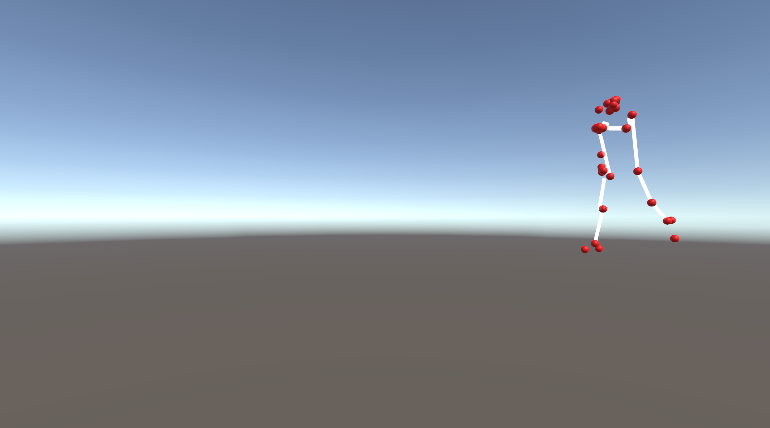
\includegraphics{1.png}
			\\[20pt]
		\end{figure}
		\begin{itemize}
			\item Popülasyon boyutu, yani her bir neslin kaç bireyden oluşacağı.
			\item Her bir genin uzunluğu. Bu örnekte genler bit dizileri olarak temsil ediliyor.
			\item Mutasyon oranı, yani her bir genin mutasyona uğrama olasılığı.
			\item  Hedef gen, yani genetik algoritmanın hedeflediği bit dizisi.
			
			
			\clearpage
			
		\end{itemize}	
	
	\item \textbf {'create population'} \\Fonksiyonu, başlangıç popülasyonunu oluşturur. Rastgele bit dizileri oluşturarak popülasyonu doldurur.\\[10pt]
	\begin{figure}[!h]
		\centering
		
\includegraphics[width=1.2\textwidth]{3.png}
		\\[20pt]
	\end{figure}
		\item \textbf {'fitness'} \\Fonksiyonu, bir genin uygunluk değerini hesaplar. Uygunluk değeri, hedef gene ne kadar yakın olduğunu belirten bir skordur.
	\begin{figure}[!h]
		\centering
		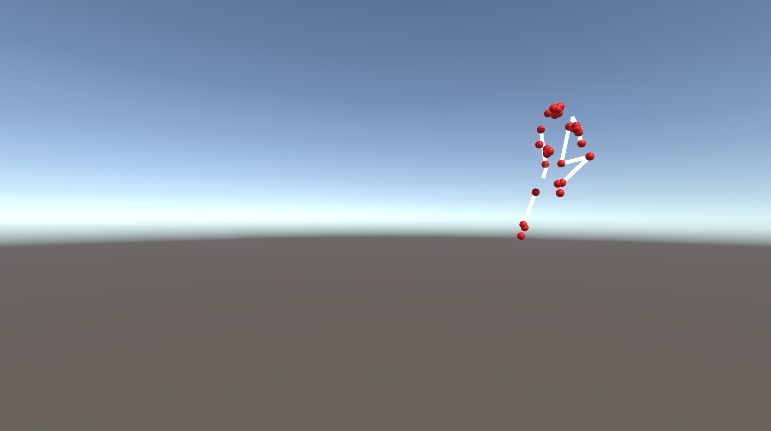
\includegraphics{4.png}
		\\[20pt]
	\end{figure}
	\newpage
		\item \textbf{rank population fonksiyonu} \\Popülasyonu uygunluk değerine göre sıralar. En yüksek uygunluk değerine sahip genler en üstte olacak şekilde sıralanır.
	\begin{figure}[!h]
		\centering
		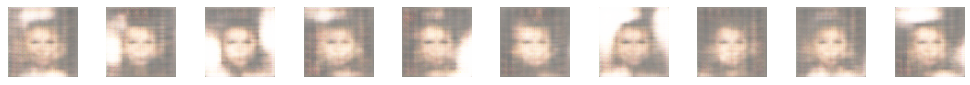
\includegraphics{5.png}
		\\[20pt]
	\end{figure}
	\item \textbf{select parents fonksiyonu} \\
	Ebeveyn seçimi yapar. Bu örnekte turnuva seçimi kullanılmıştır; rastgele iki birey seçilir ve onlardan uygunluk değeri daha yüksek olanı ebeveyn olarak seçilir
	\begin{figure}[!h]
		\centering
		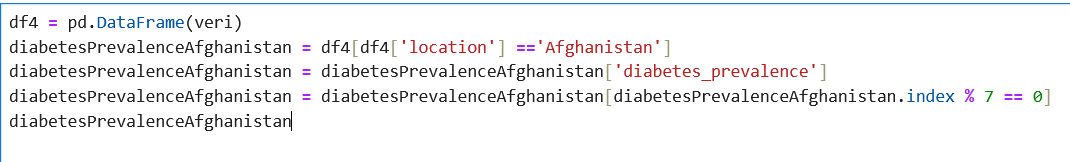
\includegraphics{6.png}
		\\[20pt]
	\end{figure}
	\item \textbf{crossover fonksiyonu}\\ Çaprazlama işlemini gerçekleştirir. İki ebeveynin genlerini alır ve belirli bir noktadan çaprazlar, böylece iki yeni çocuk gen oluşturur.
	\begin{figure}[!h]
		\centering
		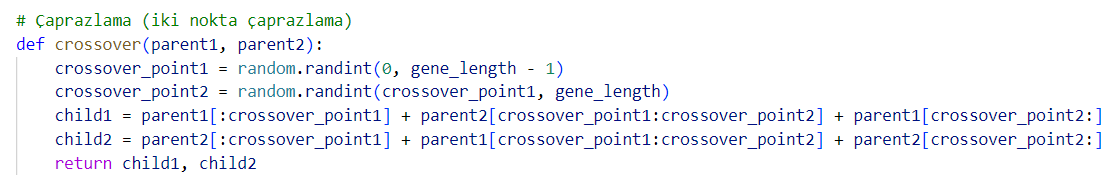
\includegraphics[width=1.2\textwidth]{7.png}
		\\[20pt]
	\end{figure}
		\clearpage
	\item \textbf{mutate fonksiyonu}\\ Genlerde mutasyon gerçekleştirir. Her bir bitin mutasyona uğrama olasılığı mutation rate parametresi tarafından belirlenir.
	\begin{figure}[!h]
		\centering
		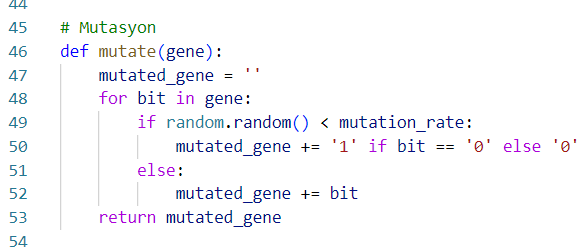
\includegraphics{8.png}
		\\[20pt]
	\end{figure}
	\item \textbf{create new generation fonksiyonu}\\Bir sonraki nesli oluşturur. Ebeveynleri seçer, çaprazlama ve mutasyon işlemlerini uygular, ve yeni nesli oluşturur.
	\begin{figure}[!h]
		\centering
		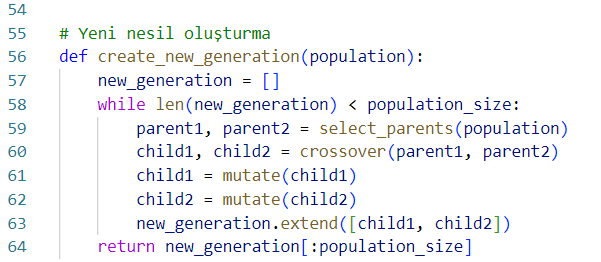
\includegraphics{9.png}
		\\[20pt]
	\end{figure}
	\newpage
	\item \textbf{genetic algorithm fonksiyonu}\\ Genetik algoritmayı çalıştırır. Başlangıç popülasyonu oluşturur, her bir nesilde en iyi geni ve uygunluk değerini gösterir, ve hedef gene ulaşılana kadar yeni nesiller oluşturur.
	\begin{figure}[!h]
		\centering
		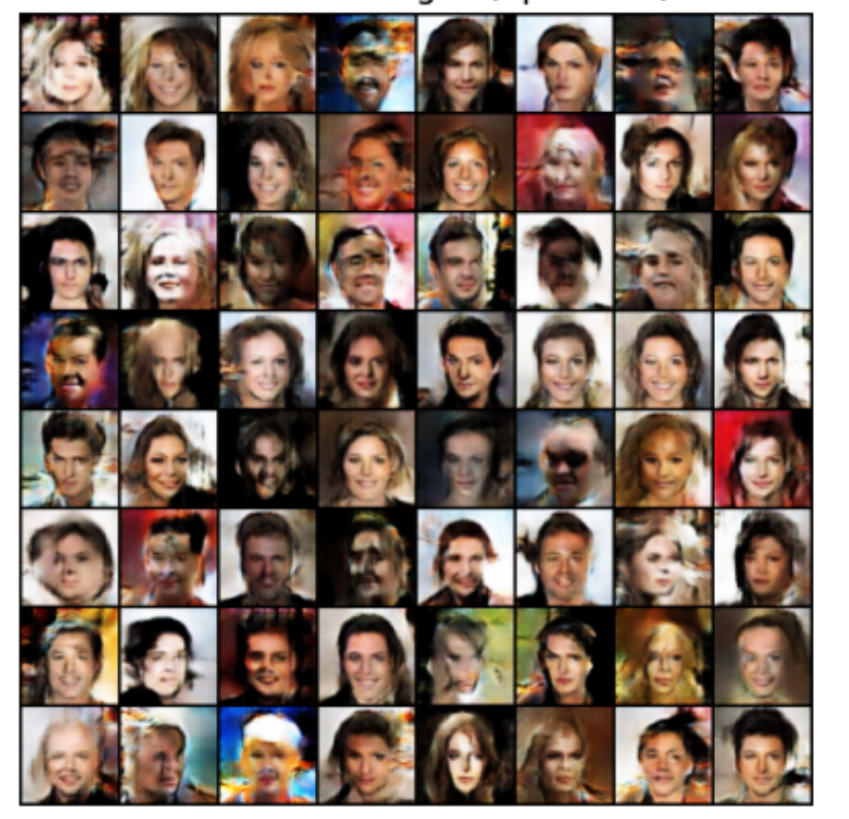
\includegraphics[width=1.2\textwidth]{10.png}
		\\[20pt]
	\end{figure}
	\item \textbf{main }\\ Genetic algorithm fonksiyonu çağrılır ve genetik algoritma çalıştırılır.
	\begin{figure}[!h]
		\centering
		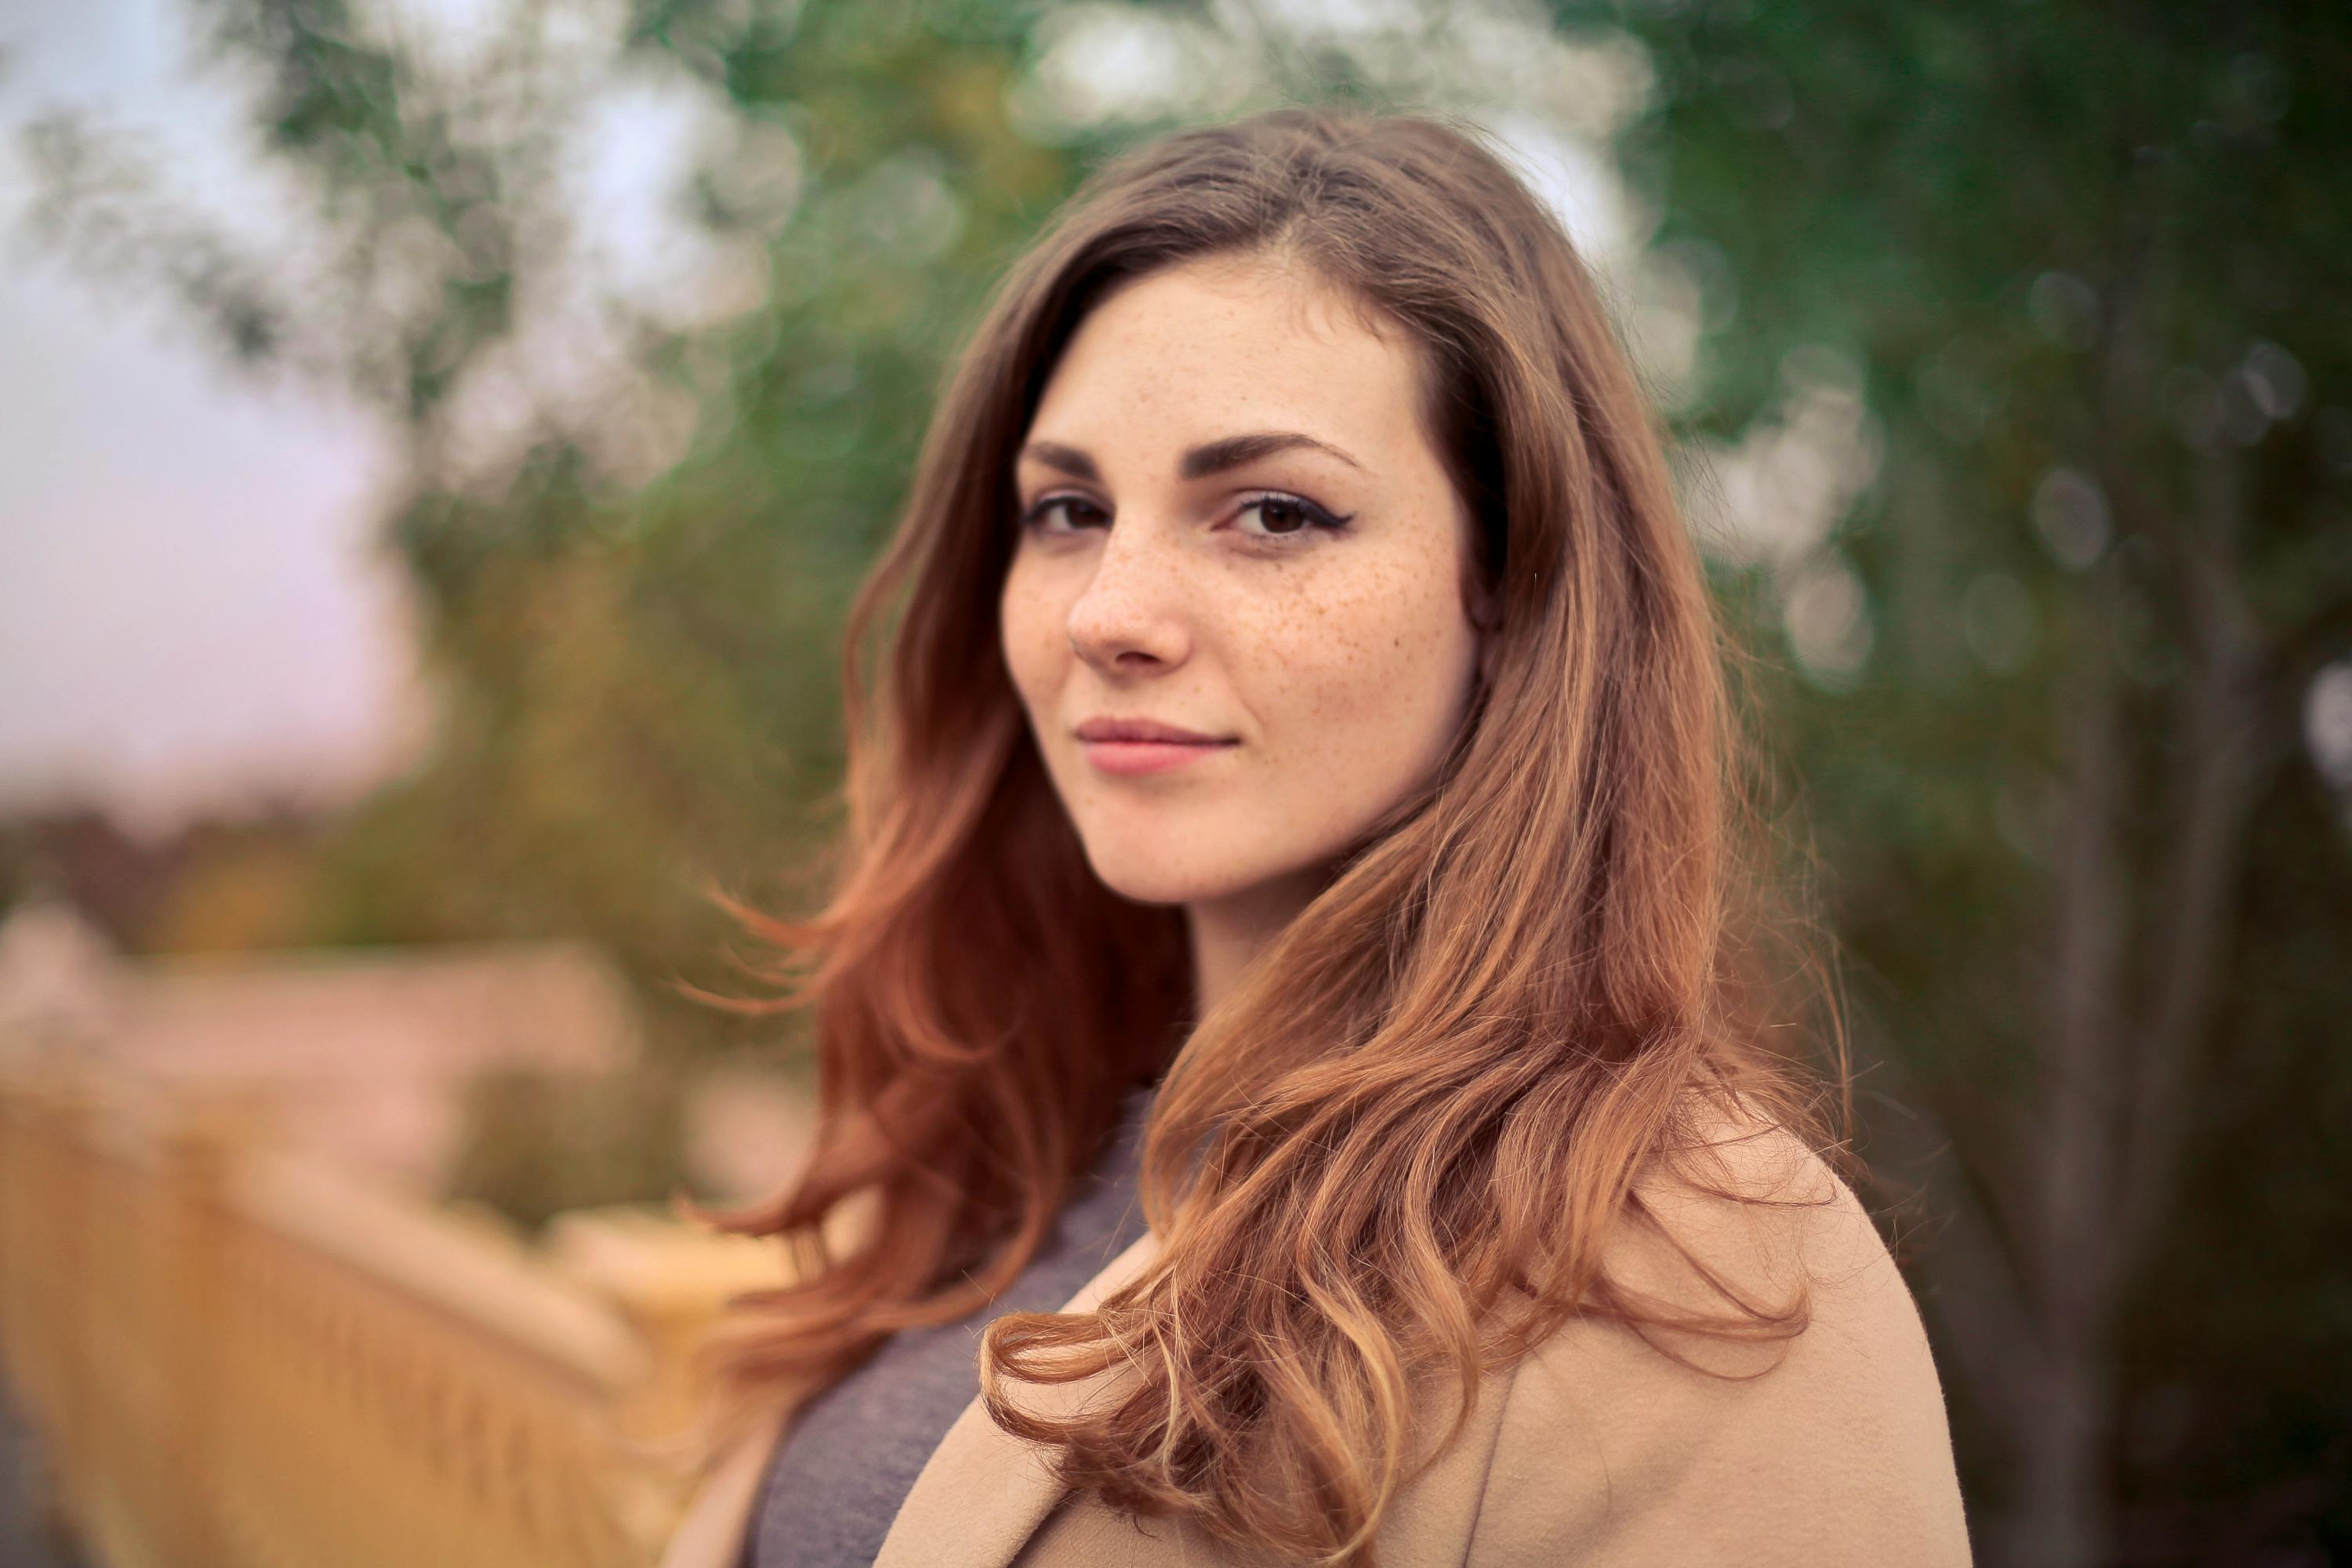
\includegraphics{11.png}
		\\[20pt]
	\end{figure}
	\\[40pt]
	
\end{enumerate}
	
	Bu adımların birleşimi, genetik algoritmanın çalışmasını sağlar. Başlangıçta rastgele bir popülasyon oluşturulur, her bir nesilde en iyi genler seçilir ve çaprazlama ve mutasyon işlemleri uygulanarak yeni nesiller oluşturulur. Bu süreç, hedef gene ulaşılana kadar devam eder.\\[20pt]
	\newpage
	
\begin{figure}[!h]
	\centering
	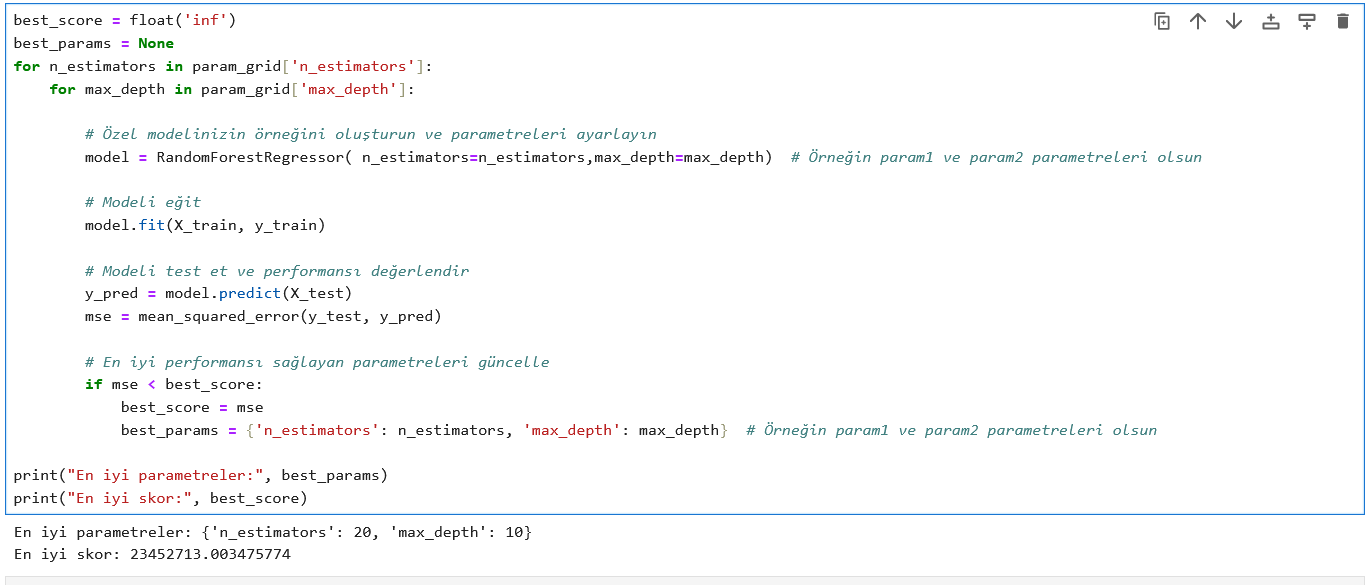
\includegraphics{12.png}
	\\[20pt]
\end{figure}
Bu çıktı, genetik algoritmanın her bir nesilindeki en iyi geni ve bu genin uygunluk değerini gösteriyor. Her bir satır, bir jenerasyonu temsil eder.\\[20pt]

Örneğin, "Generation 1, Best gene: 10001100, Fitness: 5" satırı ilk jenerasyonun en iyi genini (10001100) ve bu genin uygunluk değerini (Fitness: 5) gösterir. Daha sonra, her jenerasyonda en iyi gen ve uygunluk değeri güncellenir.\\[20pt]

Son jenerasyonda (Generation 24), hedef gen olan "10101010" elde edilmiştir ve uygunluk değeri 8'dir. Bu, genetik algoritmanın hedef gende yaklaştığını ve sonunda hedefi başarıyla bulduğunu gösterir.\\[20pt]
	
\subsection{Örnek-2}	
 Bu bölümün ikinci çalışmasında Genetik Algoritma kullanılarak 'örnek-1'adlı çalışmadan  esinlenerek  yapılmıştır.Uygulamada ki amac hedef sayısı olan 1905'ı bulmaktır.\\[20pt]


\begin{figure}[!h]
	\centering
	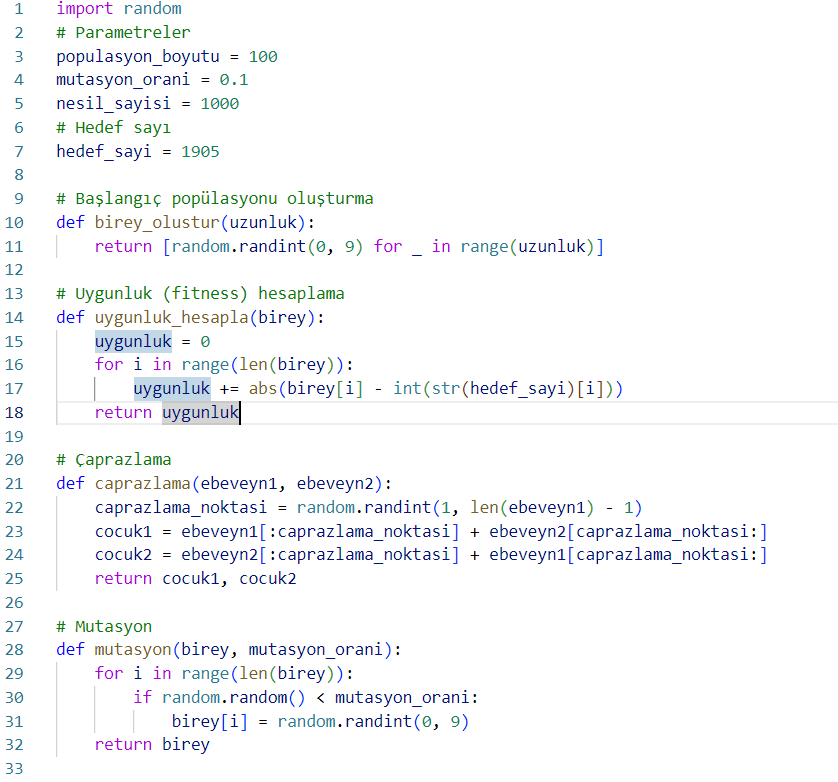
\includegraphics[width=1.2\textwidth]{33.png}
	
\end{figure}
\begin{figure}[!h]
	\centering
	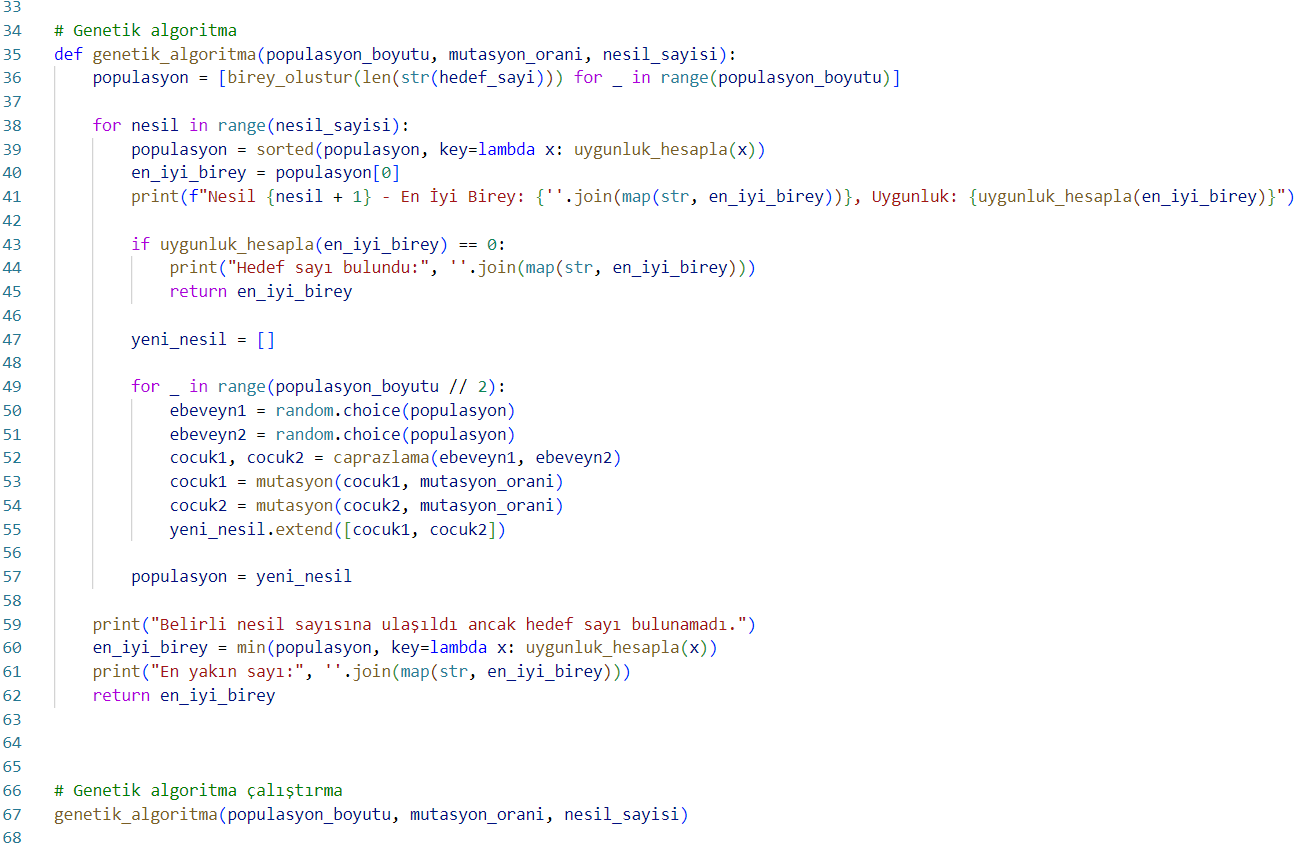
\includegraphics[width=1.3\textwidth]{34.png}
	
\end{figure}
\newpage
\begin{itemize}
	\item Parametreler: populasyon boyutu, mutasyon orani ve nesil sayisi gibi parametreler, genetik algoritmanın çalışma şeklini belirler.
	\item Hedef Sayı Belirleme: İlk olarak, hedef sayıyı 1905 olarak belirliyoruz.
	\item Başlangıç Popülasyonu Oluşturma: birey olustur fonksiyonu, belirli bir uzunluktaki bireyi rastgele oluşturur. Her bir birey, hedef sayıdaki rakamların sayısına sahip olacak şekilde 0 ile 9 arasında rastgele rakamlardan oluşur.
	\item Uygunluk (Fitness) Hesaplama: uygunluk hesapla fonksiyonu, bir bireyin hedef sayıya ne kadar uygun olduğunu hesaplar. Her bir rakamın hedef sayıdaki rakamla ne kadar uyumlu olduğunu belirlemek için mutlak değer farkları toplanır.\clearpage
	\item  Çaprazlama: caprazlama fonksiyonu, iki ebeveyn bireyden yeni çocuk bireyler üretir. Rastgele bir çaprazlama noktası belirlenir ve bu noktaya kadar olan kısımlar ebeveynler arasında değiştirilerek çocuklar oluşturulur.
	\item Mutasyon: mutasyon fonksiyonu, bir bireyin genlerinde belirli bir mutasyon oranıyla rastgele değişiklikler yapar. Her bir gen için belirli bir olasılıkla (mutasyon oranına bağlı olarak) yeni bir rastgele rakam atanır.
	\item Genetik Algoritma: genetik algoritma fonksiyonu, genetik algoritmayı uygular. Belirli bir populasyon boyutu ve nesil sayısı ile başlar. Her bir nesilde, populasyon uygunluklarına göre sıralanır ve en iyi birey ekrana yazdırılır. Eğer hedef sayı bulunursa veya belirli bir nesil sayısına ulaşılırsa döngüden çıkılır.
	
	\item Genetik Algoritma Çalıştırma: En son kısımda ise parametrelerle genetik algoritma çalıştırılır.
	
	
\end{itemize}	
\newpage

\begin{figure}[!h]
	\centering
	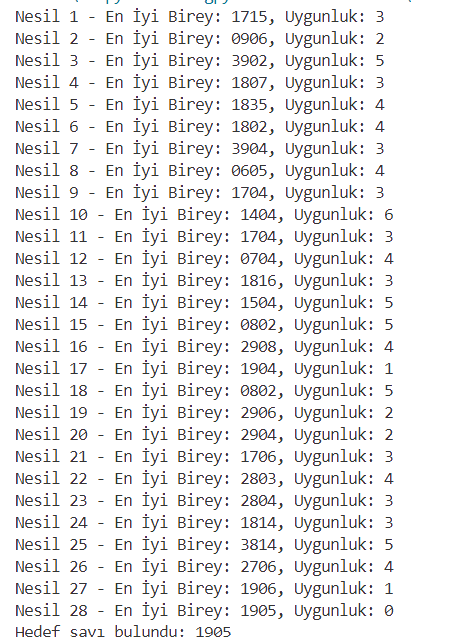
\includegraphics[width=0.7\textwidth]{cıktı.png}	 	
\end{figure}
Bu çıktı, genetik algoritmanın her neslindeki en iyi bireyi ve uygunluk değerini göstermektedir.\\
Örneğin, "Nesil 1 - En İyi Birey: 1715, Uygunluk: 3" ifadesi, ilk neslin en iyi bireyinin 1715 olduğunu ve bu bireyin uygunluk değerinin 3 olduğunu belirtir. Uygunluk değeri, hedef sayıya ne kadar yakın olduğunu gösterir. Daha küçük bir uygunluk değeri, hedef sayıya daha yakın bir çözümü temsil eder.\\
Çıktıda görüldüğü gibi, 28. nesilde uygunluk değeri 0 olan bir birey bulunmuştur. Bu, hedef sayının tam olarak bulunduğunu gösterir. Sonuç olarak, "Hedef sayı bulundu: 1905" ifadesiyle belirtilir.




\subsection{Çizelgeleme ve Genetik Algoritmalar}

Genetik algoritmaların çizelgeleme problemlerinde kullanımı, ilk olarak 1985 yılında Davis tarafından yapılmıştır. Davis'in çalışmasında, bir iş atölyesinde kârı maksimize etmek için çizelgelemenin önemi vurgulanmıştır. Bu çalışma, gerçekçi olmaktan ziyade basit ve öğretici bir çizelgeleme problemi üzerinde genetik algoritmaların nasıl uygulanabileceğini göstermiştir. Davis'in bu çalışması, sonraki araştırmalar için önemli bir temel oluşturmuştur.\\[10pt]


Genetik algoritmalar çizelgeleme problemlerinin çözümünde önemli bir rol oynamakta ve bu alanda yapılan çalışmalar, bu algoritmaların etkinliğini ve uygulanabilirliğini göstermektedir. Gelecekteki çalışmalar, genetik algoritmaların çizelgeleme problemlerindeki performansını artırmak ve daha karmaşık problemleri ele almak için yöntemlerin geliştirilmesine sağlayacaktır.\\[10pt]




Önceki bölümde genetik algoritmalar detaylı bir şekilde incelenmiş ve yapısı ile kullanım detayları üzerinde durulmuştu. Bu bölümde ise genetik algoritmaların çizelgeleme problemlerinde nasıl kullanıldığı ele alınmış ve örnek  çalışmalar özetlenmiştir.\\[10pt]


\subsubsection{Örnek-1}
Bu örneğimizde  Genetik Algoritma kullanılarak  cizelgeleme problemleri ele alınmıştır. Genetik Algoritma kullanılarak  bir Ders programı cizelgesi oluşturulmuş ve kod blokları ile detaylı olarak  açıklanmıştır.\cite{Tobs80}

	\begin{enumerate}
	\item \textbf Değişkenlerin ve İthalatların Tanımlanması:
	
	\begin{figure}[!h]
		\centering
		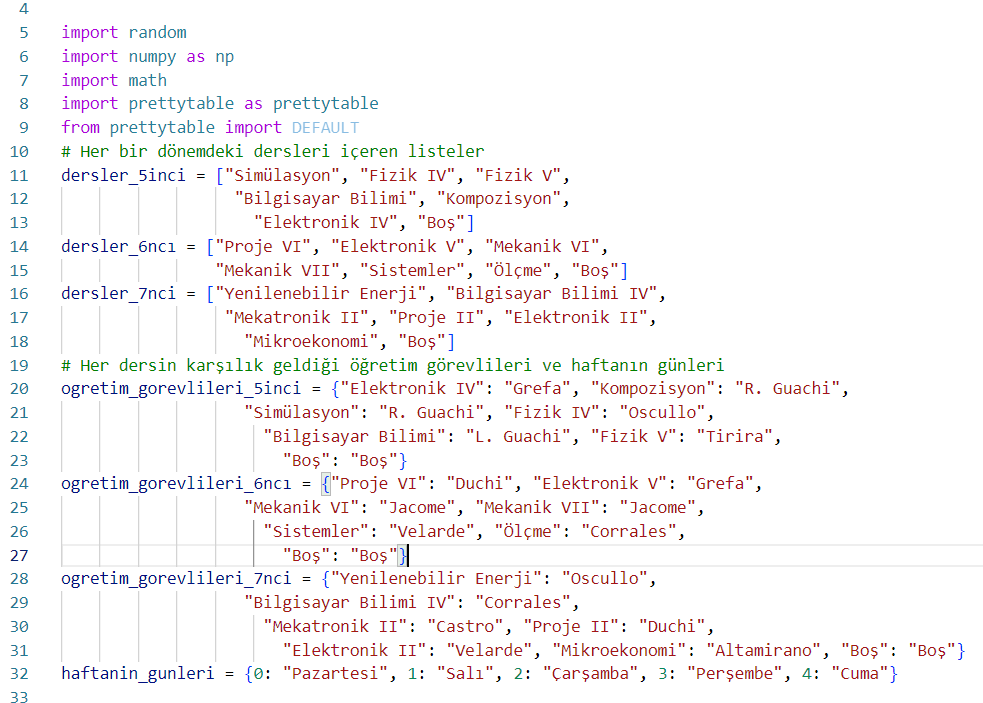
\includegraphics[width=1.2\textwidth]{5.1.png}
		\\[20pt]
	\end{figure}
	\begin{itemize}
		\item İlk olarak, kodun başında gerekli kütüphaneler random, numpy, math, ve prettytable gibi, import edilir.
		\item Ardından, dönemlerdeki dersleri içeren listeler  tanımlanır. Her bir ders listesi, ilgili dönemdeki derslerin adlarını içerir.
		
		\begin{figure}[!h]
			\centering
			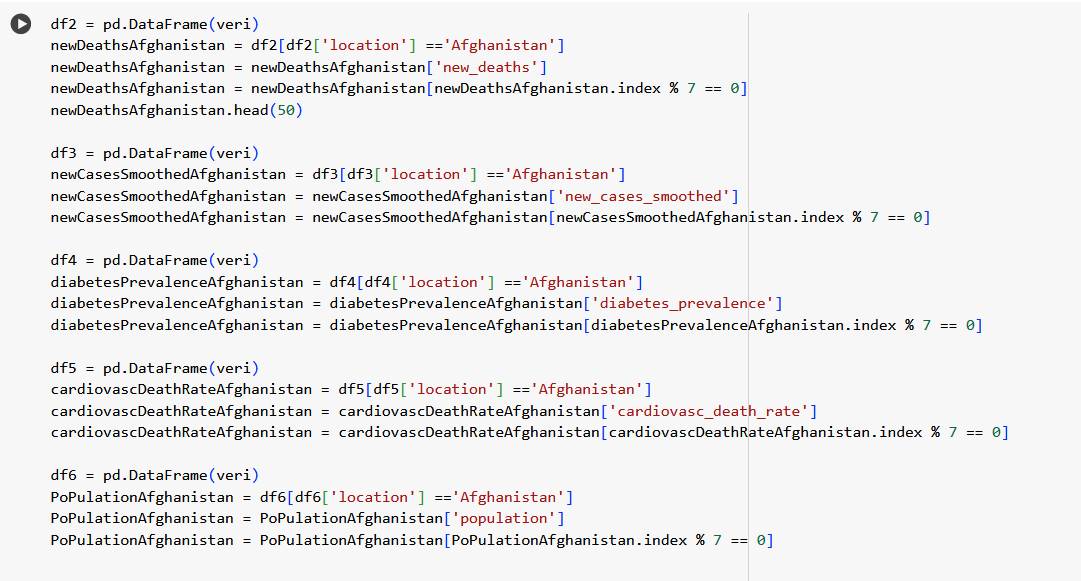
\includegraphics[width=1\textwidth]{5.3.png}
			\\[20pt]
		\end{figure}
		\item
		Popülasyon büyüklüğünü temsil eden 'populasyon', ders sayısını temsil eden 'ders sayisi' ve mutasyona uğrayan birey sayısını belirten 'mutasyona uğrayanlar' gibi değişkenler tanımlanır.
		\item Mutasyon olasılığı 'mutasyon olasılığı' ve maksimum nesil sayısı 'maksimum nesil 'değişkenleri belirlenir.
	\end{itemize}	
	\newpage
	
	\item \textbf Zaman Tablosunu Yazdırmak İçin Fonksiyon:
	\begin{itemize}
		\item \textbf{'ders programını yazdır'} fonksiyonu, bir ders programını daha okunaklı bir şekilde yazdırmak için oluşturulmuştur. Bu fonksiyon, \textbf{prettytable}'' kütüphanesini kullanarak bir tablo oluşturur ve ders programını bu tabloya doldurur.
		
		\begin{figure}[!h]
			\centering
			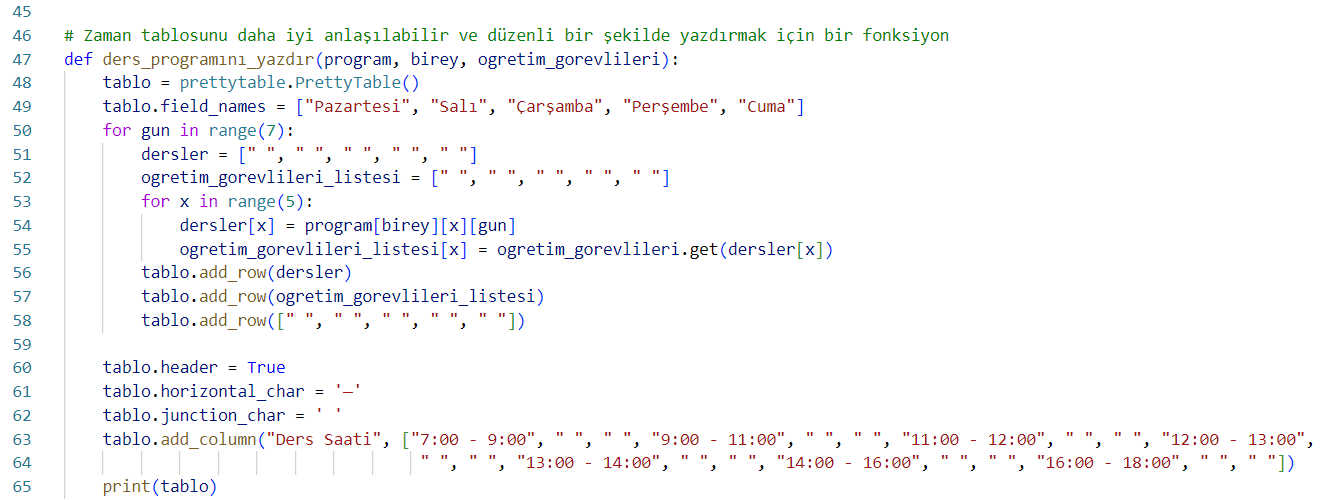
\includegraphics[width=1.3
			\textwidth]{5.4.png}
			\\[5pt]
		\end{figure}
	\end{itemize}
	\item \textbf 	Genetik Algoritmayı Kullanarak En İyi Ders Programını Bulmak İçin Fonksiyonlar:
	\begin{itemize}
		\item \textbf sıralama Fonksiyonu, bir listeyi küçükten büyüğe sıralamak için kullanılır.
		
		\begin{figure}[!h]
			\centering
			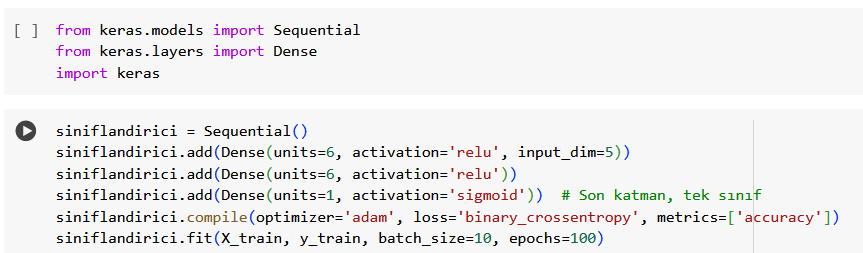
\includegraphics[width=0.9
			\textwidth]{5.5.png}
			\\[20pt]
		\end{figure}
		\newpage
		
		
		\begin{figure}[!h]
			\centering
			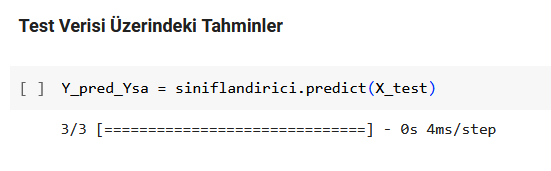
\includegraphics[width=1.3
			\textwidth]{5.6.png}
			\\[20pt]
		\end{figure}
		
		\item \textbf{PopulasyonuOlustur} fonksiyonu, başlangıç popülasyonunu oluşturur. Her bir birey, her bir günde rastgele seçilen derslerden oluşur.
		
		\item \textbf{uygunluk hesapla} fonksiyonu, bir bireyin uygunluğunu (fitness) hesaplar. Bu uygunluk, derslerin çakışma sayısına bağlıdır; yani aynı gün ve saatte aynı öğretmenin iki dersi olması durumunda uygunluk azalır.
		\newpage
		\begin{figure}[!h]
			\centering
			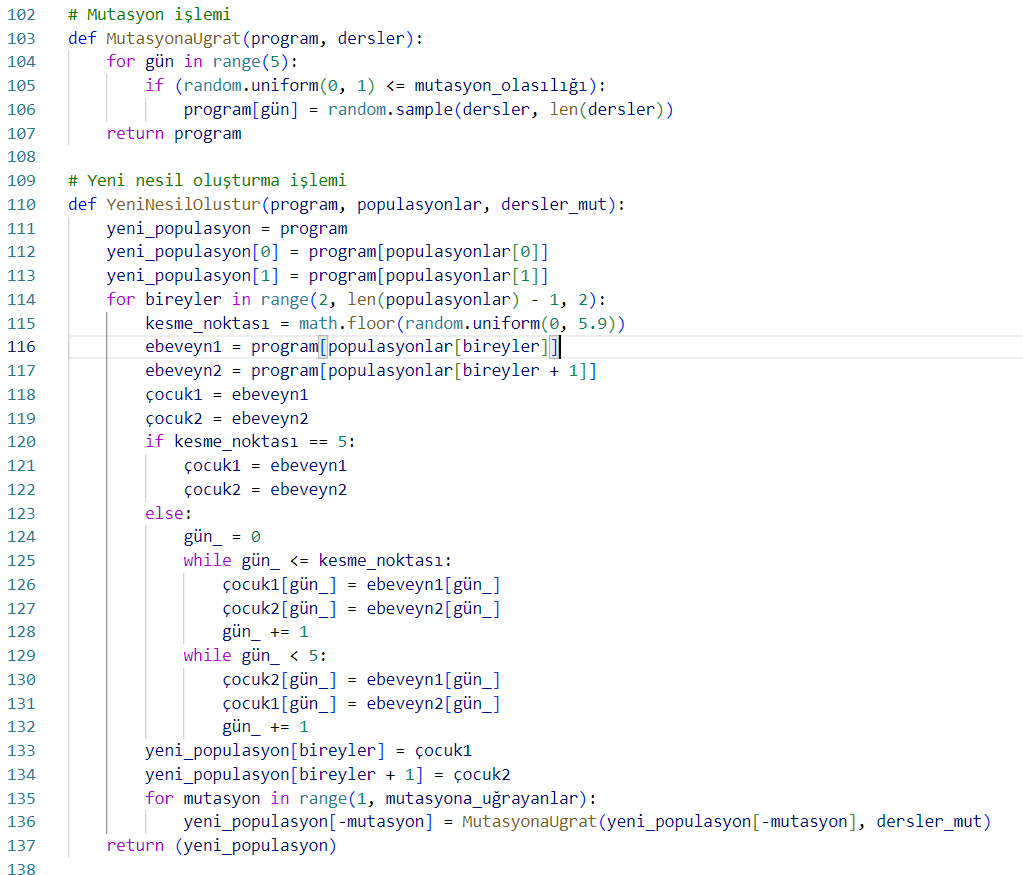
\includegraphics[width=1.2
			\textwidth]{5.7.png}
			\\[20pt]
		\end{figure}
		\item \textbf{MutasyonaUgrat} fonksiyonu, bir bireye mutasyon uygular. Mutasyon, belirli bir olasılıkla rastgele derslerin yerlerini değiştirerek gerçekleşir.
		\item \textbf{YeniNesilOlustur} fonksiyonu, bir sonraki nesli oluşturur. Bu fonksiyon, melezleme ve mutasyon operatörlerini kullanarak yeni bireyler oluşturur.
		
		
	\end{itemize}
	\newpage
	\begin{figure}[!h]
		\centering
		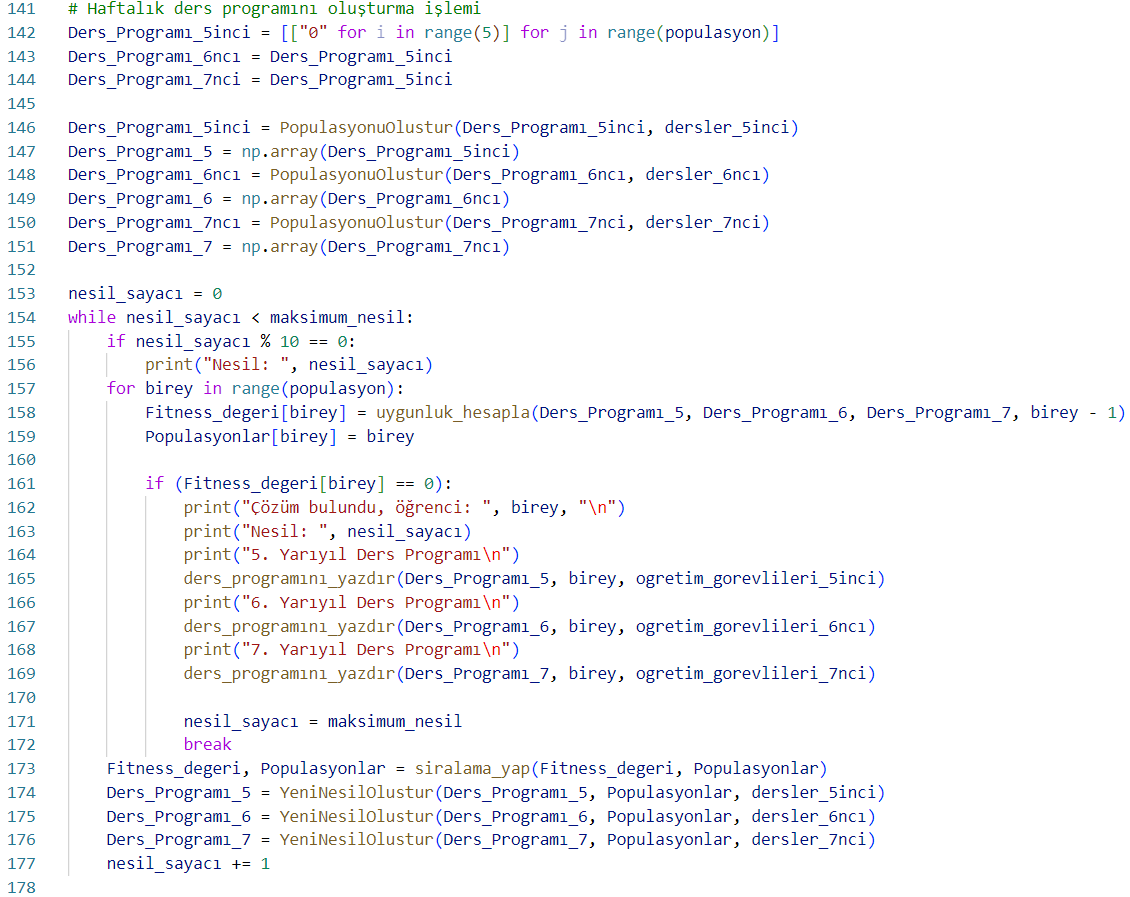
\includegraphics[width=1.22
		\textwidth]{5.8.png}
		
	\end{figure}
	
	
	\item \textbf Genetik Algoritmayı Uygulama ve En İyi Ders Programını Bulma:
	\begin{itemize}
		\item  Her bir matris, bir popülasyon büyüklüğü kadar satıra ve her bir gün için bir sütuna sahiptir. Bu matrisler, başlangıçta rastgele ders programları ile doldurulur.
		\item 'while ' döngüsü, maksimum nesil sayısına ulaşılana kadar çalışır. Her nesilde, her bir bireyin uygunluğu hesaplanır ve en uygun bireyler seçilir.
		\item Seçilen bireyler arasında çaprazlama ve mutasyon operatörleri uygulanarak yeni bir nesil oluşturulur.
		\item Her bir dönem için ayrı ayrı uygunluk hesaplamaları yapılır ve en uygun ders programı bulunduğunda, program durdurulur ve bulunan ders programı ekrana yazdırılır.
		
	\end{itemize}
	
	
	
	\begin{figure}[htbp]
		\centering
		\begin{subfigure}[b]{0.8\textwidth}
			\centering
			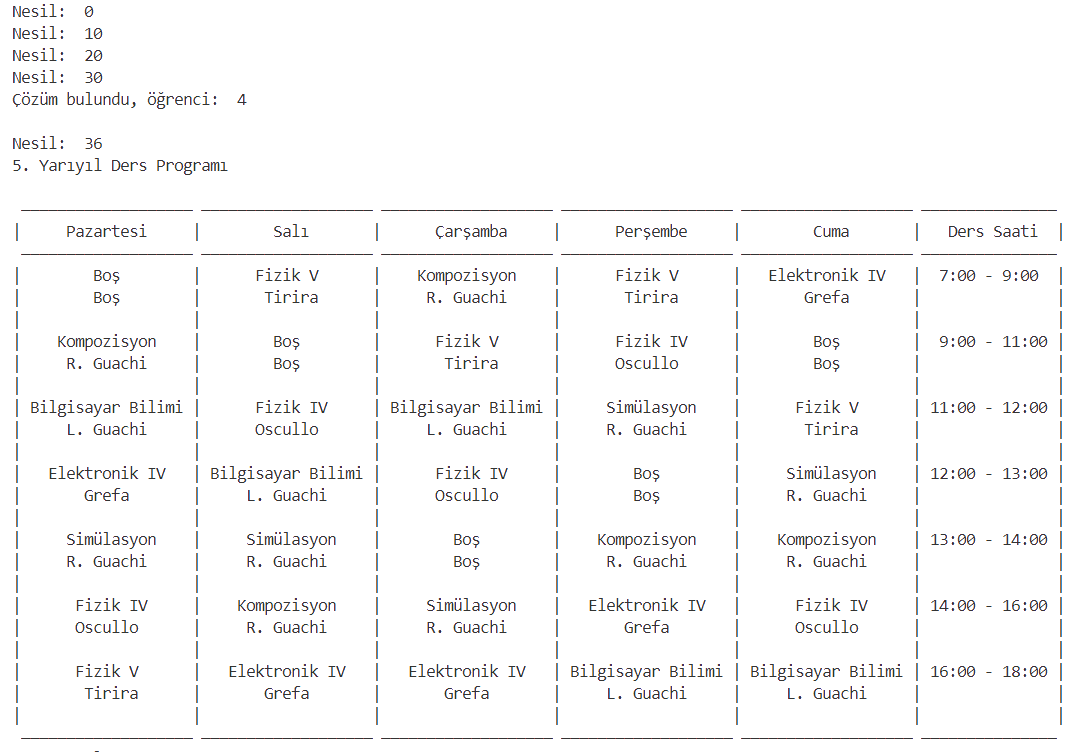
\includegraphics[width=\textwidth]{5.9.png}
			
			\label{fig:resim1}
		\end{subfigure}
		\hfill
		\begin{subfigure}[b]{0.8\textwidth}
			\centering
			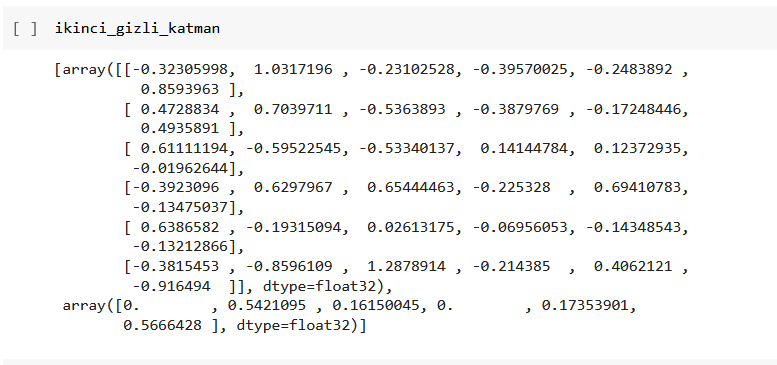
\includegraphics[width=\textwidth]{5.10.png}
			
			\label{fig:resim1}
		\end{subfigure}
		\hfill
		\begin{subfigure}[b]{0.8\textwidth}
			\centering
			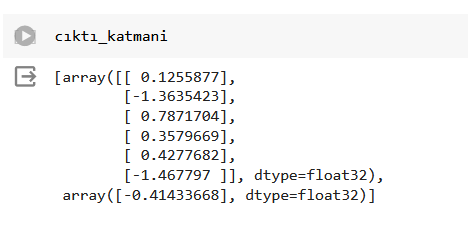
\includegraphics[width=\textwidth]{5.11.png}
			
			\label{fig:resim2}
		\end{subfigure}
		
		\label{fig:iki_resim}
	\end{figure}
	
	
	\clearpage
\end{enumerate}











\section{ Veri Ve Sistem Tasarımı}
    Bu bölümünde yapılan çalışmada kullanılan veriler ve çalışma mödelinin tasarımı detaylı olarak anlılmıştır. \\
	Çalışmada  kullanılan veriler; Ahsen KÜÇÜK'ün  hazırlamış olduğu ve Prof. Dr. İpek DEVECİ KOCAKOÇ danişmanlık yaptığı  "HEMŞİRE ÇİZELGELEME PROBLEMLERİNİN GENETİK ALGORİTMALARLA OPTİMİZASYONU VE BİR UYGULAMA" başlıklı yüksek lisans tez çalışmasında kullanılan Buca Seyfi Demirsoy Devlet Hastanesi, Koroner Yoğun Bakım servisinin Şubat 2015 çizelgeleridir.\cite{kuccuk2021hemcsire}
	\\[40pt]







\subsection{Hemşire Nöbet Çizelgeleme Problemi}
\item Hemşire nöbet çizelgesi problemi, sağlık sektöründe kaynakların verimli kullanımı ve kaliteli hasta bakımı sağlanması açısından büyük önem taşıyan bir çizelgeleme problemidir. Bu problem, hemşirelerin vardiya saatlerinin düzenlenmesi ve hastanenin 24 saat kesintisiz hizmet vermesini sağlamak amacıyla, karmaşık kısıtlar ve hedeflerin optimize edilmesini gerektirir.\\[5pt]
\item Hemşire nöbet çizelgesi problemi, sağlık hizmetlerinin sürekliliğini ve kalitesini sağlamak için kritik bir öneme sahiptir. Bu problemin etkin bir şekilde çözülmesi, hemşirelerin iş yükünü dengelerken hastaların ihtiyaç duyduğu kesintisiz bakımı sağlamaya yardımcı olur. Optimizasyon teknikleri ve özellikle genetik algoritmalar, bu süreçte önemli bir rol oynayarak, hastane yönetimlerine ve sağlık çalışanlarına büyük faydalar sağlar.


 


	\subsection{Hemşire Nöbet Cizelgeleme Problemi Test Mödeli}
	
	Bölümde Genetik algoritmalar ile  bir Test modeli tasarlanmıştır.Test modelimizde 5 hemşirenin, 7 günlük içinde ve  2 vardiya şeklinde nöbet çizelgesi oluşturulmuş ve tablo şeklinde gösterilmiştir.Amaç modelimizin çalışmasını ve sonuclarını gözlemlemektir.Bu sayede sistemin Gerçek mödel de daha iyi çalışması amaçlanmıştır.
	
\subsubsection{Parametrelerin Tanımlanması:} n, m, k, u, ve h gibi parametreler belirtilir. Bunlar sırasıyla hemşire sayısı, gün sayısı, vardiya sayısı, uzman hemşire sayısı ve gece nöbetine kalmayacak hemşire sayısıdır.

\begin{figure}[!h]
	\centering
	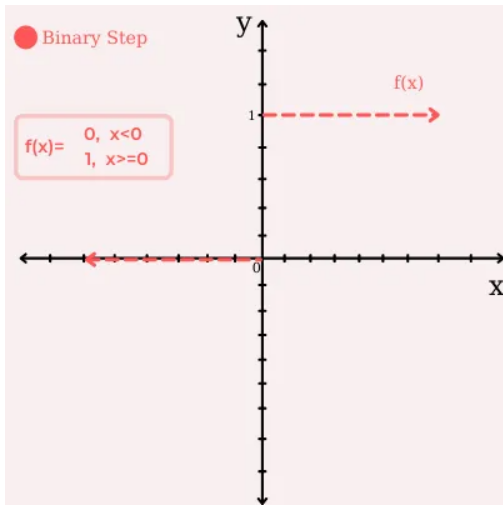
\includegraphics[width=1.2\textwidth]{6.1.png}
	
\end{figure}

\subsubsection{Genetik Algoritmanın Oluşturulması} GenetikAlgoritma adında bir sınıf tanımlanır. Bu sınıf, genetik algoritmanın bütün özelliklerini içerir.
\subsubsection{Amaç Fonksiyonunun Tanımlanması: }'amac fonksiyonu' metodu, bireylerin uygunluk değerlerini hesaplar. Bu uygunluk değerleri, çalışma sürelerinin minimize edilmesine yönelik bir amaç fonksiyonu kullanılarak elde edilir.Amaç fonksiyonu, her bir bireyin ne kadar iyi olduğunu ölçer, her bir bireyin toplam çalışma süresi hesaplanır.


\subsubsection{Başlangıç Popülasyonunun Oluşturulması:}'populasyon olustur' metodu kullanılarak başlangıç popülasyonu oluşturulur. Her birey, bir vardiyadaki her hemşirenin her gün için bir vardiya yapmasını temsil eden bir genotip içerir. Genetik algoritma bir başlangıç popülasyonu ile başlar. Her bir birey, problemdeki bir çözümü temsil eder.Her bir birey bir hemşirenin her bir gün için vardiya yapma durumunu temsil eder. Başlangıç popülasyonu, rastgele seçilen genlerden oluşur.

\begin{figure}[!h]
	\centering
	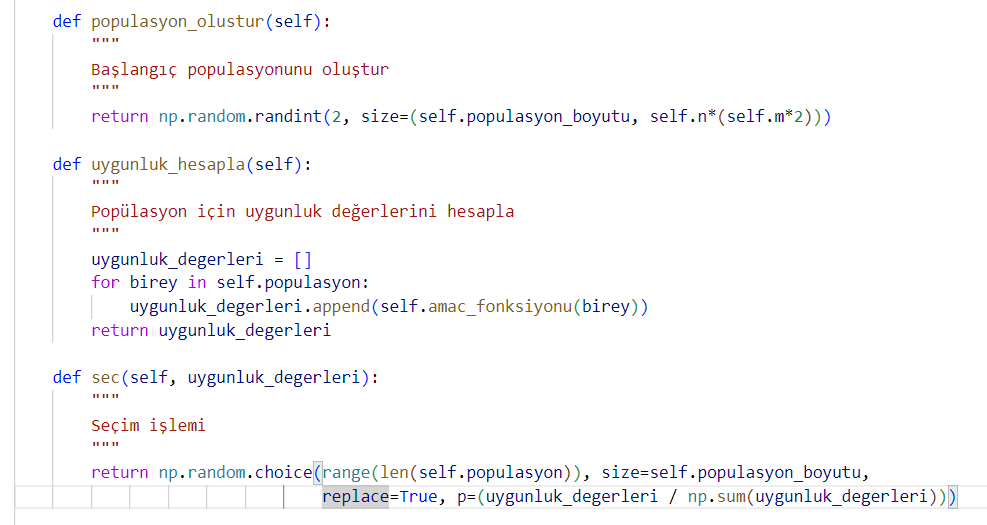
\includegraphics[width=1.2\textwidth]{6.2.png}
	\\[20pt]
\end{figure}


\subsubsection{Seçim İşlemi: }Popülasyon içindeki bireylerin uygunluk değerlerine göre seçim yapılır. Daha uygun bireyler, daha büyük bir olasılıkla seçilir. Bu, daha iyi çözümlerin gelecek nesillere aktarılmasını sağlar.
\begin{figure}[!h]
	\centering
	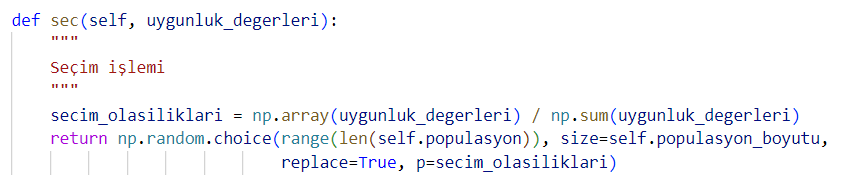
\includegraphics[width=1.2\textwidth]{6sec.png}
	\\[20pt]
\end{figure}
\newpage
\subsubsection{Kısıtların Tanımlanması}kisitlar metodu, problemdeki kısıtları tanımlar..  Her hemşirenin bir günde en fazla bir vardiya yapması, uzman hemşirelerin her gün en az bir vardiya yapması ve gece nöbetine kalmayacak hemşirelerin her gün gece vardiyası yapmaması gibi kısıtlar belirlenir.\\
\begin{figure}[!h]
	\centering
	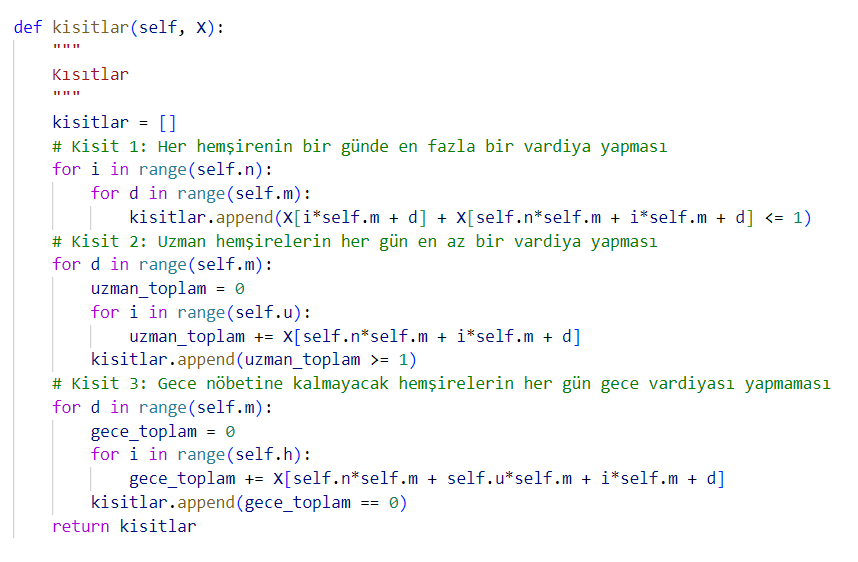
\includegraphics[width=1.2\textwidth]{6.3.png}
	\\[20pt]
\end{figure}
Problemdeki kısıtlar, hemşirelerin çalışma düzenini belirler
\clearpage
\subsubsection{Çaprazlama İşlemi ve Mutasyon İşlemi: }'caprazla' metodu, seçilen bireyler arasında çaprazlama işlemi gerçekleştirilir. Bu işlem, iki bireyin genetik materyalinin bir kısmının birbiriyle değiştirilmesini sağlar. Yeni bireyler, ebeveynlerin özelliklerini taşıyan ancak farklılıklar içeren çocuklar olur.\\'mutasyon' metodu, Yeni bireylerde mutasyon işlemi uygulanır. Bu, rastgele seçilen genlerin değerlerinin değiştirilmesini içerir. Bu, çeşitliliği arttırır ve potansiyel olarak daha iyi çözümlerin bulunmasına yardımcı olur..
\begin{figure}[!h]
	\centering
	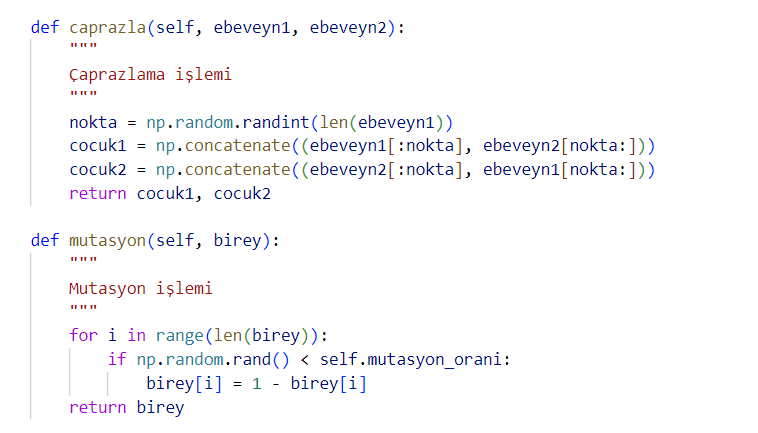
\includegraphics[width=1.2\textwidth]{6.4.png}
	\\[20pt]
\end{figure}

Yeni nesil bireylerin oluşturulması için seçim, çaprazlama ve mutasyon işlemleri uygulanır
\newpage
\subsubsection{Optimizasyonun Gerçekleştirilmesi: }'optimize et' metodu, genetik algoritmayı belirli bir maksimum nesil sayısına kadar çalıştırır ve en iyi çözümü bulur.
\begin{figure}[!h]
	\centering
	\includegraphics[width=1.2\textwidth]{6.5.png}
	\\[20pt]
\end{figure}\\
Belirli bir nesil sayısı veya başka bir durum sağlandığında optimizasyon işlemi sonlandırılır. En iyi çözüm, amaç fonksiyonunun en küçük olduğu birey olarak belirlenir.
\newpage
\subsubsection{Sonuçların Gösterilmesi:} En iyi çözüm ve uygunluk değerleri gösterilir. Bu, problemdeki en iyi çözümün ne olduğunu ve bu çözümün ne kadar iyi olduğunu belirtir.

\begin{figure}[!h]
	\centering
	\includegraphics[width=1.2\textwidth]{6.6.png}
	\\[20pt]
\end{figure}
\subsubsection{Cıktı} Belirtilen kısıtlamalar  ve amac fonksiyonu ile  hemşirelerin calışma saatlerini minimuma indirip ,oluşturulabilecek en optimum sonucu burada gösterilmektedir. 

\begin{figure}[!h]
	\centering
	\includegraphics[width=0.8\textwidth]{6cıktı2.png}
	\\[20pt]
\end{figure}

\begin{table}
	\begin{flushleft}
		\caption{Test Çalışması Sonuç Tablosu}
	\end{flushleft}
	
\begin{tabular}{l|l|l|}
	
	\rowcolor{yellow}
	Hemşire & Tarih & Vardiya  \\
	\hline
	Hemşire 1  & 2024-05-30 Perşembe  &  İzinli  \\
	Hemşire	2 & 2024-05-30 Perşembe & Gece  \\
	Hemşire	3 & 2024-05-30 Perşembe & Gündüz \\
	Hemşire	4 & 2024-05-30 Perşembe & İzinli \\
	Hemşire	5 & 2024-05-30 Perşembe & Gece \\
	\rowcolor{yellow}
	\hline Hemşire & Tarih & Vardiya  \\
	\hline
	Hemşire 1  & 2024-05-31 Cuma  &  Gündüz  \\
	Hemşire	2 & 2024-05-31 Cuma & İzinli  \\
	Hemşire	3 & 2024-05-31 Cuma & Gündüz\\
	Hemşire	4 & 2024-05-31 Cuma & Gece \\
	Hemşire	5 & 2024-05-31 Cuma & İzinli\\
	\rowcolor{yellow}
	\hline Hemşire & Tarih & Vardiya  \\
	\hline
	Hemşire 1  & 2024-06-01 Cumartesi  &  Gündüz  \\
	Hemşire	2 & 2024-06-01 Cumartesi & Gece  \\
	Hemşire	3 & 2024-06-01 Cumartesi & Gündüz \\
	Hemşire	4 & 2024-06-01 Cumartesi & İzinli \\
	Hemşire	5 & 2024-06-01 Cumartesi & Gece \\
	\rowcolor{yellow}
	\hline Hemşire & Tarih & Vardiya  \\
	\hline
	Hemşire 1  & 2024-06-02 Pazar  &  Gündüz  \\
	Hemşire	2 & 2024-06-02 Pazar & Gece  \\
	Hemşire	3 & 2024-06-02 Pazar & Gündüz \\
	Hemşire	4 & 2024-06-02 Pazar & Gece \\
	Hemşire	5 & 2024-06-02 Pazar & İzinli \\
	\rowcolor{yellow}
	\hline Hemşire & Tarih & Vardiya  \\
	\hline
	Hemşire 1  & 2024-06-03 Pazartesi  &  Gece  \\
	Hemşire	2 & 2024-06-03 Pazartesi & İzinli  \\
	Hemşire	3 & 2024-06-03 Pazartesi & Gündüz \\
	Hemşire	4 & 2024-06-03 Pazartesi & İzinli \\
	Hemşire	5 & 2024-06-03 Pazartesi & Gece \\
	\rowcolor{yellow}
	\hline Hemşire & Tarih & Vardiya  \\
	\hline
	Hemşire 1  & 2024-06-04 Salı  &  İzinli  \\
	Hemşire	2 & 2024-06-04 Salı & Gece  \\
	Hemşire	3 & 2024-06-04 Salı & İzinli \\
	Hemşire	4 &2024-06-04 Salı & Gündüz \\
	Hemşire	5 & 2024-06-04 Salı & Gece \\
	\rowcolor{yellow}
	\hline Hemşire & Tarih & Vardiya  \\
	\hline
	Hemşire 1  & 2024-06-05 Çarşamba  &  Gece  \\
	Hemşire	2 & 2024-06-05 Çarşamba & İzinli  \\
	Hemşire	3 & 2024-06-05 Çarşamba & Gece \\
	Hemşire	4 & 2024-06-05 Çarşamba& Gündüz \\
	Hemşire	5 & 2024-06-05 Çarşamba & İzinli \\
\end{tabular}

\end{table}




\newpage



\subsection{Hemşire Nöbet Çizelgeleme Problemi Mödel Sistem Tasarımı}


\subsubsection{Parametrelerin Tanımlanması:}
\item Hemşire nöbet çizelgesi probleminin başarılı bir şekilde çözülmesi için, ilgili parametrelerin dikkatlice tanımlanması gerekmektedir. Parametreler, problemin yapısını ve çözüm sürecini belirleyen temel unsurlardır.\\[5pt]
\item Çalışmada  n, m, k, u, ve h gibi parametreler belirtilir. Bunlar sırasıyla hemşire sayısı, gün sayısı, vardiya sayısı, uzman hemşire sayısı ve gece nöbetine kalmayacak hemşire sayısıdır.\\[10pt]
\item GenetikAlgoritma sınıfı, hemşire vardiyası optimizasyon problemi için bir çerçeve sağlar. Bu sınıf, problemle ilgili parametreleri ve yöntemleri içerir.\\[10pt]
\item 'init' yöntemi, sınıfın başlatıcı yöntemidir. Bu yöntem, problemde kullanılacak parametreleri alır ve başlangıç popülasyonunu oluşturur.\\[10pt]


\begin{figure}[!h]
	\centering
	\includegraphics[width=1.2\textwidth]{8.1.png}
	
\end{figure}

\newpage

\subsubsection{Amaç Fonksiyonunun Tanımlanması: }
\item Amaç fonksiyonu, çizelgeleme problemlerinin çözümünde belirli bir hedefe ulaşmayı sağlayan matematiksel bir ifadedir. Bu fonksiyon, problemin çözüm sürecinde hangi kriterlerin optimize edileceğini belirler.
\item Bu fonksiyon, çözümün etkinliğini ve başarısını belirleyen temel unsurlardan biridir. Doğru ve uygun bir amaç fonksiyonunun tanımlanması, problemin istenilen şekilde çözülmesini sağlar ve elde edilen çözümlerin kalite seviyesini artırır. Dolayısıyla, çizelgeleme algoritmalarının tasarımında amaç fonksiyonunun dikkatlice seçilmesi ve optimize edilmesi gerekmektedir.
\item Çalışmamız da 'amac fonksiyonu' metodu, bireylerin uygunluk değerlerini hesaplar. Bu uygunluk değerleri, çalışma sürelerinin minimize edilmesine yönelik bir amaç fonksiyonu kullanılarak elde edilir.Amaç fonksiyonu, her bir bireyin ne kadar iyi olduğunu ölçer, her bir bireyin toplam çalışma süresi hesaplanır.\\[10pt]

\begin{equation}
	\label{eq:1}
	\text{Minimize} \quad \sum_{i=0}^{n-1} \sum_{d=0}^{m-1} \left( 8 \cdot X_{i \cdot m + d} + 16 \cdot X_{n \cdot m + i \cdot m + d} \right)
\end{equation}

Denklem \ref{eq:1} ,Çalışma sürelerinin en aza indirilmesi sağlamaktadır.

\begin{figure}[!h]
	\centering
	\includegraphics[width=1.2\textwidth]{8.2.png}
	
\end{figure}

\subsubsection{Kısıtların Tanımlanması:}
\item Kısıtlar, belirli görevlerin veya işlemlerin yerine getirilmesi sırasında karşılaşılan sınırlamaları ve zorunlulukları ifade eder.
\newpage
\item Kısıtların önemi, çizelgeleme problemlerinin çözüm sürecinde ortaya çıkar. Kısıtlar, çözümün geçerliliğini belirleyen temel unsurlar olduğundan, bu kısıtların ihlal edilmesi durumunda elde edilen çözümler pratikte uygulanamaz hale gelir. Dolayısıyla, çizelgeleme algoritmalarının tasarımında kısıtların dikkatlice ele alınması ve çözüm sürecine entegre edilmesi gerekmektedir.

\item Çalışmamız da "kisitlar" fonksiyonu  ile problemdeki kısıtları tanımlar.
Problemdeki kısıtlar, hemşirelerin çalışma düzenini belirler.\\ 
Bu kısıtlar, her hemşirenin günlük maksimum vardiya sayısı, uzman hemşirelerin her gün en az bir vardiya yapması gibi kuralları içerir.\\[10pt]

\item Uygulamada kullanılan  kısıtların  denklem karşılıkları aşağıda verilmiştir



\begin{equation}
	\label{eq:2}
	X_{i,d} + X_{n \cdot m + i \cdot m + d} \leq 1 \quad \forall i, \forall d
\end{equation}
Denklem \ref{eq:2} ,Her hemşire bir günde en fazla bir vardiya yapabilir kısıtını sağlamaktadır 

\begin{equation}
	\label{eq:3}
	\sum_{i=0}^{u-1} X_{n \cdot m + i \cdot m + d} \geq 1 \quad \forall d
\end{equation}
Denklem  \ref{eq:3} ,Uzman hemşirelerin her gün en az bir vardiya yapması kısıtını sağlamaktadır  \\[10pt]
\begin{equation}
	\label{eq:4}
	\sum_{i=0}^{h-1} X_{n \cdot m + u \cdot m + i \cdot m + d} = 0 \quad \forall d
\end{equation}
Denklem  \ref{eq:4}, Gece nöbetine kalmayacak hemşirelerin her gün gece vardiyası yapmaması kısıtını sağlamaktadır \\[10pt]
\begin{equation}
	\label{eq:5}
	X_{i,d} + X_{n \cdot m + i \cdot m + d} \leq 1 \quad \forall i, \forall d
\end{equation}
Denklem  \ref{eq:5}, Gündüz vardiyasında çalışan bir hemşirenin gece vardiyasında çalışmaması kısıtını sağlamaktadır  \\[10pt]
\begin{equation}
	\label{eq:6}
	\sum_{i=0}^{n-1} X_{n \cdot m + i \cdot m + d} = 2 \quad \forall d
\end{equation}
Denklem \ref{eq:6} ,Her hemşire nöbetçi olmadığı gün 8 saat çalışır. Haftada 40 saat, ayda 160 saat çalışma zorunluluğu kısıtını sağlamaktadır  \\[10pt]

\begin{equation}
	\label{eq:7}
	\sum_{d=0}^{m-1} \left[ 8 (1 - X_{i,d}) + 16 X_{n \cdot m + i \cdot m + d} \right] = saat \quad \forall i
\end{equation}
Denklem  \ref{eq:7},	Akşam nöbeti tutanlara ertesi gün görev verilmez kısıtını sağlamaktadır  \\[10pt]
\begin{equation}
	\label{eq:8}
	X_{i,d} + X_{n \cdot m + i \cdot m + d} \leq 1 \quad \forall i, \forall d
\end{equation}
Denklem \ref{eq:8}, Hemşire aynı gün içinde yalnızca bir vardiyada çalışabilir ya da izinlidir kısıtını sağlamaktadır   \\[10pt]
\begin{equation}
	\label{eq:9}
	X_{i,d} + X_{n \cdot m + i \cdot m + d} \leq 1 \quad \forall i, \forall d
\end{equation}
Denklem \ref{eq:9}, Akşam vardiyasında nöbet tutan iki kişiden birinin uzman olması kısıtını sağlamaktadır \\[10pt]
\begin{equation}
	\label{eq:10}
	\sum_{i=0}^{u-1} X_{n \cdot m + i \cdot m + d} \geq 1 \quad \forall d
\end{equation}
Denklem \ref{eq:10}	, Sabah vardiyasında çalışan hemşire akşam vardiyasında çalışmayacak	kısıtını sağlamaktadır \\[10pt]		
\begin{equation*}
	\label{eq:11}
	X_{i,d} + X_{n \cdot m + i \cdot m + d} \leq 1 \quad \forall i, \forall d
\end{equation*}
Denklem	\ref{eq:11}, Uzman hemşireler gece vardiyasında en az bir kişi olmalı kısıtını sağlamaktadır \\[10pt]				
\begin{equation}
	\label{eq:12}
	\sum_{i=0}^{u-1} X_{n \cdot m + i \cdot m + d} \geq 1 \quad \forall d
\end{equation}
Denklem	 \ref{eq:12}, Gece nöbetine kalmayacak hemşireler kısıtını sağlamaktadır\\[10pt]				
\begin{equation}
	\label{eq:13}
	\sum_{i=0}^{h-1} X_{n \cdot m + u \cdot m + i \cdot m + d} = 0 \quad \forall d
\end{equation}
Denklem	 \ref{eq:13} ,Gece nöbetinde iki kişi çalışır (kısıtlı olanlar hariç)	kısıtını sağlamaktadır \\[20pt]			
\begin{equation}
	\label{eq:14}
	\sum_{i=0}^{n-1} X_{n \cdot m + i \cdot m + d} = 2 \quad \forall d
\end{equation}
Denklem	  \ref{eq:14},	Ayda en az 160 saat calışma kısıtını sağlayan denklem kısıtını sağlamaktadır\\[20pt]
\begin{equation}
	\label{eq:15}
	\sum_{d=0}^{m-1} \left[ 8 X_{i,d} + 16 X_{n \cdot m + i \cdot m + d} \right] \geq 160 \quad \forall i
\end{equation}
Denklem	 \ref{eq:15}, Ayda en az 160 saat çalışmalı kısıtını sağlayan denklem kısıtını ssağlamaktadır \\[20pt]
\begin{equation}
	\label{eq:16}
	X_{n \cdot m + i \cdot m + d} + X_{i,d+1} = 0 \quad \forall i, \forall d < m
\end{equation}
Denklem	 \ref{eq:16} ,Gece nöbet tutan ertesi gün gündüz çalışmaz kısıtını sağlayan denklem kısıtını sağlamaktadır
\\[50pt]
\item Extra olarak uygulamada kullanılan  kısıtların  kod satırlarının resimleri  aşağıda verilmiştir.Her bir kısıt için yorum satırları oluşturulmuş ve bilgisi verilmiştir.
\begin{figure}[htbp]
	\centering
	\begin{subfigure}[b]{1\textwidth}
		\centering
		\includegraphics[width=\textwidth]{8kısıt1.png}
		
		\label{fig:resim1}
	\end{subfigure}
	\hfill
	\begin{subfigure}[b]{1.\textwidth}
		\centering
		\includegraphics[width=\textwidth]{8kısıt2.png}
		
		\label{fig:resim1}
	\end{subfigure}
	\hfill
	
\end{figure}
\newpage
\begin{figure}[htbp]
	\centering
	\begin{subfigure}[b]{1\textwidth}
		\centering
		\includegraphics[width=\textwidth]{8kısıt3.png}
		
		
	\end{subfigure}
	\hfill
	\begin{subfigure}[b]{1\textwidth}
		\centering
		\includegraphics[width=\textwidth]{8kısıt4.png}
		
		
	\end{subfigure}
	\hfill
	
\end{figure}
\clearpage

\subsubsection{Uygunluk Değerlerinin Hesaplanması: }

\item Genetik algoritmalar, çizelgeleme problemleri gibi karmaşık optimizasyon problemlerinin çözümünde etkili bir yöntem olarak öne çıkmaktadır. Bu algoritmaların başarısında uygunluk değeri (fitness value) önemli bir rol oynar. Uygunluk değeri, her bir çözüm adayının (bireyin) problemde belirlenen amaç fonksiyonuna ne kadar iyi uyduğunu ölçen bir metriktir
\item Genetik algoritmalarda uygunluk değeri, çözüm sürecinin merkezinde yer alır. Uygunluk değeri, çözümlerin kalitesini ölçer, doğal seleksiyon sürecine rehberlik eder, genetik çeşitliliği korur ve optimizasyon hedeflerini dengelemeye yardımcı olur. Bu nedenle, uygunluk değeri, genetik algoritmaların etkinliğini ve başarısını belirleyen kritik bir faktördür.\\ Çizelgeleme problemlerinin çözümünde, uygunluk değerinin doğru ve etkili bir şekilde tanımlanması, algoritmanın performansını ve elde edilen çözümlerin kalitesini önemli ölçüde artırır.

\item Çalışmamız da "uygunluk hesapla yöntemi", her bireyin uygunluk değerini hesaplar. Bu değerler, bireylerin amaca ne kadar uygun olduğunu gösterir.\\[10pt]



\begin{figure}[!h]
	\centering
	\includegraphics[width=1.2\textwidth]{8uygunluk.png}
	
\end{figure}
\subsubsection{Seçim İşlemi}

\item Genetik algoritmalarda seçim işlemi (selection process) büyük bir öneme sahiptir çünkü bu işlem, hangi bireylerin bir sonraki nesilde daha fazla temsil edileceğini belirler. Seçim işlemi, popülasyonun genel kalitesini artırarak optimizasyon sürecinin etkinliğini ve hızını doğrudan etkiler.\\
Ayrıca, optimizasyon hedeflerine ulaşmada ve dengeli çözümler bulmada önemli bir rol oynar. Bu nedenle, genetik algoritmaların başarısı ve etkinliği büyük ölçüde seçim işleminin doğru ve etkili bir şekilde gerçekleştirilmesine bağlıdır.
\item Çalışmamız da "sec yöntemi", seçim işlemini gerçekleştirir. Bu işlem, uygunluk değerlerine göre bireyleri seçer. Daha uygun bireylerin seçilme olasılığı daha yüksektir.



\begin{figure}[!h]
	\centering
	\includegraphics[width=1.2\textwidth]{8sec.png}
	
\end{figure}



\subsubsection{Çaprazlama İşlemi ve Mutasyon İşlemi: }
\item Çaprazlama ve mutasyon, genetik algoritmaların temel bileşenleri olup, optimizasyon süreçlerinde genetik çeşitliliği artırarak daha iyi çözümler bulunmasını sağlar. Çaprazlama, genetik materyalin karıştırılması yoluyla yeni çözümler üretirken, mutasyon genetik çeşitliliği koruyarak ve lokal minimumlardan kaçınarak çözüm alanının genişlemesine yardımcı olur. Bu işlemler, genetik algoritmaların etkinliğini ve başarısını önemli ölçüde artırır.
\item Çalışmamız da "caprazla" metodu, seçilen bireyler arasında çaprazlama işlemi gerçekleştirilir. Bu işlem, iki bireyin genetik materyalinin bir kısmının birbiriyle değiştirilmesini sağlar. Yeni bireyler, ebeveynlerin özelliklerini taşıyan ancak farklılıklar içeren çocuklar olur.\\[10pt]
\item Ayrıca "mutasyon" metodu ile  Yeni bireylerde mutasyon işlemi uygulanır. Bu, rastgele seçilen genlerin değerlerinin değiştirilmesini içerir. Bu, çeşitliliği arttırır ve potansiyel olarak daha iyi çözümlerin bulunmasına yardımcı olur.\\[10pt]


\begin{figure}[!h]
	\centering
	\includegraphics[width=1.2\textwidth]{8cap.mut.png}
	\\[20pt]
\end{figure}

\item	Yeni nesil bireylerin oluşturulması için seçim, çaprazlama ve mutasyon işlemleri uygulanır	

\newpage


\subsubsection{Optimizasyonun Gerçekleştirilmesi: }
Optimizasyon, belirli bir hedefe ulaşmak için en iyi çözümün bulunmasını amaçlayan matematiksel ve hesaplamalı bir süreçtir.
Genetik algoritmalar, çizelgeleme problemlerinin optimizasyonunda kritik bir role sahiptir. Karmaşık ve çok boyutlu problemlerin çözümünde, esnek ve adaptif yapılarıyla, global optimuma ulaşma yetenekleriyle ve çok kriterli optimizasyon kapasiteleriyle öne çıkarlar.\\[10pt]
\item Çalışmamız da "optimize et" metodu, genetik algoritmayı belirli bir maksimum nesil sayısına kadar çalıştırır ve en iyi çözümü bulur.
\item Ayrıca "optimize et" yöntemi, genetik algoritmayı çalıştırır. Bu yöntem, belirli bir nesil sayısı boyunca seçim, çaprazlama ve mutasyon işlemlerini tekrarlar. Her iterasyonda, uygunluk değerleri daha iyiye doğru ilerler.\\[10pt]
\begin{figure}[!h]
	\centering
	\includegraphics[width=1.2\textwidth]{8optimize.png}
	
\end{figure}
\newpage
\item 	Belirli bir nesil sayısı veya başka bir durum sağlandığında optimizasyon işlemi sonlandırılır. En iyi çözüm, amaç fonksiyonunun en küçük olduğu birey olarak belirlenir.\\[10pt]
\newpage
\subsubsection{Sonuçların Gösterilmesi:} 
\item En iyi çözüm ve uygunluk değerleri gösterilir. Bu, problemdeki en iyi çözümün ne olduğunu ve bu çözümün ne kadar iyi olduğunu belirtir.

\begin{figure}[!h]
	\centering
	\includegraphics[width=0.7\textwidth]{8son.png}
	
\end{figure}
\subsubsection{Cıktı}
\item Belirtilen kısıtlamalar  ve amac fonksiyonu ile  hemşirelerin calışma saatlerini minimuma indirip ,oluşturulabilecek en optimum sonucu burada gösterilmektedir.\\[10pt]
Uygunluk değeri en yüksek olan birey cıktı olarak alınır .\\[5pt]
Sonuçlar bir tablo şeklinde extra olarak gösterilmektedir.\\[5pt]

\begin{figure}[htbp]
	\centering
	\begin{subfigure}[b]{0.8\textwidth}
		\centering
		\includegraphics[width=\textwidth]{8hafta1.png}
		
		\label{fig:resim1}
	\end{subfigure}
	\hfill
	\begin{subfigure}[b]{0.8\textwidth}
		\centering
		\includegraphics[width=\textwidth]{8hafta2.png}
		
		\label{fig:resim1}
	\end{subfigure}
	\hfill
	\begin{subfigure}[b]{0.8\textwidth}
		\centering
		\includegraphics[width=\textwidth]{8hafta3.png}
		
		\label{fig:resim1}
	\end{subfigure}
	\hfill
	\begin{subfigure}[b]{0.8\textwidth}
		\centering
		\includegraphics[width=\textwidth]{8hafta4.png}
		
		
	\end{subfigure}
	\hfill
\end{figure}

\begin{center}
	\begin{landscape}
		
		
		\begin{table}
			\caption{Şubat Ayı 01.02.2015 ve 07.02.2015 Tarihleri Arası (1 Haftalık )Nöbet Cizelgesi}
			\begin{tabular}{|p{3cm}||p{2cm}||p{2cm}||p{3cm}||p{3cm}||p{3cm}||p{3cm}||p{2cm}|c|c|c|c|c|c|c|c|}
				\rowcolor{red}
				
				\hline \multicolumn{8}{|c|}{Şubat Ayı Hafta - 1} \\
				\rowcolor{yellow}
				\hline  & 01.02.2015 & 02.02.2015 & 03.02.2015 & 04.02.2015&05.02.2015&06.02.2015& 07.02.2015 \\
				\rowcolor{lightgray}
				
				\hline Hemşireler   & Pazartesi& Salı & Çarşamba & Perşembe &Cuma&Cumartesi &Pazar\\
				\hline Hemşireler 1 &  izinli & 08`16  & izinli &  08`16  &  08`16  & 08`16   &  16`08 \\
				\hline Hemşireler 2 &  izinli & 08`16  & 16`08  &  08`16  &  08`16  & 08`16   &  08`16 \\
				\hline Hemşireler 3 &  08`16  & 16`08  & 08`16  &  08`16  &  16`08  & 16`08   &  08`16 \\
				\hline Hemşireler 4 &  08`16  & 08`16  & izinli &  16`08  &  08`16  & izinli  &  izinli \\
				\hline Hemşireler 5 &  16`08  & 16`08  & izinli &  08`16  &  08`16  & izinli  &  08`16 \\
				\hline Hemşireler 6 &  izinli & 16`08  & izinli &  08`16  &  izinli & 08`16   &  izinli \\
				\hline Hemşireler 7 &  08`16  & 08`16  & 08`16  &  08`16  &  16`08  & 08`16   &  08`16 \\
				\hline Hemşireler 8 &  16`08  & 16`08  & 08`16  &  16`08  &  08`16  & 08`16   &  08`16 \\
				\hline Hemşireler 9 &  08`16  & 08`16  & 08`16  &  izinli &  08`16  & 08`16   &  08`16 \\
				\hline Hemşireler 10 & 16`08  & 08`16  & 08`16  &  08`16  &  08`16  & 16`08   &  08`16 \\
				\hline Hemşireler 11 & 08`16  & 08`16  & 08`16  &  izinli &  16`08  & 16`08   &  16`08 \\
				\hline Hemşireler 12 & 08`16  & 16`08  & 16`08  &  izinli &  08`16  & 16`08   &  16`08 \\
				\hline Hemşireler 13 & 08`16  & 08`16  & 08`16  &  08`16  &  izinli & 08`16   &  16`08 \\
				\hline Hemşireler 14 & 16`08  & izinli & 08`16  &  izinli & izinli &  08`16   &  izinli \\
				\hline
				
			\end{tabular}
			
		\end{table}
		
		\begin{table}
			\caption{{Şubat Ayı 08.02.2015 ve 14.02.2015  Tarihleri Arası (1 Haftalık ) Nöbet Cizelgesi}}
			\begin{tabular}{|p{3cm}||p{2cm}||p{2cm}||p{3cm}||p{3cm}||p{3cm}||p{3cm}||p{2cm}|c|c|c|c|c|c|c|c|}
				\rowcolor{red}
				
				\hline \multicolumn{8}{|c|}{Şubat Ayı Hafta - 2} \\
				\rowcolor{yellow}
				\hline  & 08.02.2015 & 09.02.2015 & 10.02.2015 & 11.02.2015& 12.02.2015&13.02.2015& 14.02.2015 \\
				\rowcolor{lightgray}
				\hline Hemşireler   & Pazartesi& Salı & Çarşamba & Perşembe &Cuma&Cumartesi &Pazar\\
				
				\hline Hemşireler 1 &  16`08  &  08`16 & 16`08  &  08`16  &  08`16  &   08`16   &   izinli \\
				\hline Hemşireler 2 &  08`16  &  08`16 & 08`16  &  08`16  &  08`16  &   izinli  &   08`16 \\
				\hline Hemşireler 3 &  izinli &  16`08 & izinl i&  08`16  &  16`08  &   izinli  &   16`08 \\
				\hline Hemşireler 4 &  08`16  &  16`08 & 08`16  &  08`16  &  08`16  &   izinli  &   08`16 \\
				\hline Hemşireler 5 &  16`08  &  08`16 & 16`08  &  08`16  &  izinli &   izinli  &   izinli \\
				\hline Hemşireler 6 &  izinli &  16`08 & 16`08  &  08`16  &  16`08  &   16`08   &   08`16 \\
				\hline Hemşireler 7 &  08`16  &  08`16 & 08`16  &  izinli &  08`16  &   16`08   &   izinli \\
				\hline Hemşireler 8 &  08`16  &  08`16 & 16`08  &  08`16  &  16`08  &   08`16   &   08`16 \\
				\hline Hemşireler 9 &  izinli &  08`16 & 08`16  &  08`16  &  08`16  &   16`08   &   08`16 \\
				\hline Hemşireler 10 & 16`08  &  08`16 & 08`16  &  16`08  &  izinli &   16`08   &   08`16 \\
				\hline Hemşireler 11 & 08`16  &  izinli& 08`16  &  izinli &  08`16  &   izinli  &   16`08 \\
				\hline Hemşireler 12 & izinli &  08`16 &  08`16 &  08`16  &  izinli &   izinli  &   08`16 \\
				\hline Hemşireler 13 & 16`08  &  08`16 &  16`08 &  izinli &  08`16  &   08`16   &   izinli \\
				\hline Hemşireler 14 & 08`16  &  08`16 &  16`08 &  izinli &  08`16  &   16`08   &   08`16 \\
				\hline
				
			\end{tabular}
			
		\end{table}
		
		
		\begin{table}
			\caption{Şubat Ayı 15.02.2015 ve 21.02.2015  Tarihleri Arası (1 Haftalık ) Nöbet Cizelgesi}
			
			\begin{tabular}{|p{3cm}||p{2cm}||p{2cm}||p{3cm}||p{3cm}||p{3cm}||p{3cm}||p{2cm}|c|c|c|c|c|c|c|c|}
				\rowcolor{red}
				
				\hline \multicolumn{8}{|c|}{Şubat Ayı Hafta - 3} \\
				\rowcolor{yellow}
				\hline  & 15.02.2015 & 16.02.2015 & 17.02.2015 & 18.02.2015&19.02.2015&20.02.2015& 21.02.2015 \\
				\rowcolor{lightgray}
				
				\hline Hemşireler   & Pazartesi& Salı & Çarşamba & Perşembe &Cuma&Cumartesi &Pazar\\
				
				\hline Hemşireler 1 & izinli & 08`16  & 08`16  & 08`16 & 16`08 & izinli &  izinli \\
				\hline Hemşireler 2 & 08`16  &  izinli& 08`16  & 08`16 & 08`16 & izinli &  16`08 \\
				\hline Hemşireler 3 & 08`16  &  08`16 & 08`16  & izinli& 08`16 & 16`08  &  08`16 \\
				\hline Hemşireler 4 & 08`16  &  08`16 & izinli & 08`16 & 08`16 & izinli &  izinli \\
				\hline Hemşireler 5 & 08`16  &  08`16 & 08`16  & 08`16 & 08`16 & 08`16  &  08`16 \\
				\hline Hemşireler 6 & 08`16  &  08`16 & 16`08  & 08`16 & 08`16 & 08`16  &  16`08 \\
				\hline Hemşireler 7 & 16`08  &  08`16 & 16`08  & 08`16 & 16`08 & 08`16  &  08`16 \\
				\hline Hemşireler 8 & 08`16  &  08`16 & izinli & 16`08 & 08`16 & izinli &  08`16 \\
				\hline Hemşireler 9 & 08`16  &  08`16 & 08`16  & 16`08 & 08`16 & izinli &  08`16 \\
				\hline Hemşireler 10 & 08`16 &  08`16 & izinli & 08`16 & 08`16 & 08`16  &  16`08 \\
				\hline Hemşireler 11 & 08`16 &  16`08 & 08`16  & izinli& 08`16 & 08`16  &  08`16 \\
				\hline Hemşireler 12 & 08`16 &  16`08 & 08`16  & izinli& izinli& 08`16  &  izinli \\
				\hline Hemşireler 13 & 16`08 &  16`08 & 08`16  & 08`16 & 08`16 & 08`16  &  16`08 \\
				\hline Hemşireler 14 & izinli&  08`16 & izinli & 08`16 & izinli& 08`16  &  08`16 \\
				\hline
			\end{tabular}
			
		\end{table}
		
		
		\begin{table}
			\caption{Şubat Ayı 22.02.2015 ve 28.02.2015 Tarihleri Arası (1 Haftalık ) Nöbet Cizelgesi}
			\begin{tabular}{|p{3cm}||p{2cm}||p{2cm}||p{3cm}||p{3cm}||p{3cm}||p{3cm}|p{2cm}|c|c|c|c|c|c|c|c|}
				\rowcolor{red}
				
				\hline \multicolumn{8}{|c|}{Şubat Ayı Hafta - 4} \\
				\rowcolor{yellow}
				\hline  & 22.02.2015 & 23.02.2015 & 24.02.2015 & 25.02.2015&26.02.2015&27.02.2015& 28.02.2015 \\
				\rowcolor{lightgray}
				
				\hline Hemşireler   & Pazartesi& Salı & Çarşamba & Perşembe &Cuma&Cumartesi &Pazar\\
				\hline Hemşireler 1 &  08`16 &  16`08 &  16`08 & izinli&  08`16 & 16`08 & 08`16 \\
				\hline Hemşireler 2 &  izinli&  08`16 &  08`16 & 16`08 &  08`16 & 08`16 & 08`16 \\
				\hline Hemşireler 3 &  08`16 &  08`16 &  izinli& 08`16 &  08`16 & 16`08 & 08`16 \\
				\hline Hemşireler 4 &  08`16 &  08`16 &  izinli& 08`16 &  08`16 & 08`16 & 16`08 \\
				\hline Hemşireler 5 &  izinli&  16`08 &  08`16 & 16`08 &  izinli& izinli& 08`16 \\
				\hline Hemşireler 6 &  08`16 &  16`08 &  izinli& 08`16 &  08`16 & 08`16 & 08`16 \\
				\hline Hemşireler 7 &  16`08 &  08`16 &  08`16 & 16`08 &  08`16 & 16`08 & 08`16 \\
				\hline Hemşireler 8 &  izinli&  08`16 &  08`16 & 08`16 &  08`16 & 08`16 & 08`16 \\
				\hline Hemşireler 9 &  08`16 &  izinli&  izinli& 16`08 &  izinli& 08`16 & 16`08 \\
				\hline Hemşireler 10 & 08`16 &  08`16 &  08`16 & 08`16 &  08`16 & 08`16 & 08`16  \\
				\hline Hemşireler 11 & 08`16 &  izinli&  08`16 & izinli&  08`16 & izinli& izinli \\
				\hline Hemşireler 12 & 08`16 &  08`16 &  08`16 & 08`16 &  08`16 & izinli& 08`16  \\
				\hline Hemşireler 13 & 16`08 &  16`08 &  08`16 & 16`08 &  08`16 & izinli& izinli \\
				\hline Hemşireler 14 & 08`16 &  izinli&  08`16 & izinli&  08`16 & 08`16 & 16`08  \\
				\hline
			\end{tabular}
			
		\end{table}
		
		
	\end{landscape}
\end{center}







\section{Bulgular ve Tartışma }

Sezgisel algoritmalar 
genellikle en iyiye yakın olan çözüm yoluna hızlı ve kolay şekilde ulaştıklarından, çalışmada sezgisel algoritmalardan biri olan Genetik Algoritma (GA) kullanılmıştır. Genetik Algoritmaların(GA), birden fazla optimal çözüm elde etmesi, çok sayıda parametre ile çalışma imkanı olması ve amaç fonksiyonunu geniş bir açıda araştırması nedeniyle tercih edilmiştir.\\
Çalışmamızda ilk olarak, çizelgeleme problemlerinde kısıtların çözümünün geçerliliğini belirleyen temel unsurlar olduğu kabul edilmiş ve bu nedenle kısıtları belirlenmişti. Kısıtların hastane yönetiminin amaçlarına, personel isteklerine ve yasal düzenlemelere uygun olmasına özen gösterilmiştir.\\

Genetik algoritmalar detaylı bir şekilde incelenmiş ve temel kavramlar hakkında bilgiler edinilmiştir. Bu sayede modelimizin  doğru adımlar ile  oluşturulması sağlanmıştır.\\

Modelimizin optimal sonuçlar vermesi için tasarımında amaç fonksiyonu, genetik algoritmaların popülasyon yönetimi, çaprazlama, mutasyon gibi bileşenler göz önünde bulundurulmuş ve uygulanmıştır. Ayrıca uygunluk (Fitness) değerlerine göre en optimal çözümlerin elde edilmesi için gerekli işlemler yapılarak ve model tasarlanmıştır.\\

Çalışmamızda geliştirdiğimiz test modeli üzerinde, test verileri kullanılarak çizelgeleme yapılmış ve uygunluk değerleriyle sonuçlar değerlendirilmiş ve gözlemlennmiştir.\\

Ardından gerçek veriler ve detaylı kısıtlar dikkate alınarak 28 günlük bir planlama yapılmiş ve elde edilen sonuçlar rapor edilmiştir.\\

Bu süreç, hem teorik hem de pratik açıdan genetik algoritmaların çizelgeleme problemlerindeki etkinliğini göstermiştir. İleriye dönük çalışmalarda, farklı optimizasyon teknikleri ve daha karmaşık kısıtların nasıl ele alınabileceği üzerinde durulabilir, bu da sağlık hizmetlerinde ve diğer endüstriyel uygulamalarda daha geniş bir kullanım alanı sağlayabilir.\\

\section{Sonuç}

Çizelgeleme problemlerinde, insan faktörü sebebiyle hesaplanamayacak çoklukta parametre 
görünse bile yeterli sayıda matematiksel kısıt yardımıyla gerçek modele çok yakın sonuçlar 
geliştirilebilir. Büyük boyutlu ve doğrusal olmayan kısıtların olduğu çizelgeleme 
problemlerinde  GA kullanımı da standart 
çözücülerin kullanıldığı durumdan farksız olup etkin olmayacaktır. Sonuç olarak; farklı sezgisel algoritmaların 
da kullanılacağı hibrit yaklaşımlar daha etkin çözümler verebilir. \\





\begin{center}
	TEŞEKKÜRLER

 \end{center}
\begin{center}
	Başta her daim yanımızda olan, değerli bilgi ve birikimi ile her türlü desteği gösteren Sayın Emre GÜNGÖR hocama ve dönem boyunca her hafta birbirinden değerli  sunumlar yaparak 
	kendi konularını üzerinde bizlere farkındalık oluşturmaya çalışan tüm arkadaşlarıma 
	teşekkürlerimi sunarım..
\end{center}











	
	
	
	

	

\end{flushleft}
	%Kaynakçayı yazdırmak
\bibliographystyle{ieeetr}
\bibliography{references.bib} 
%\printbibliography %Prints bibliography



\end{document}	